\documentclass[12 pt]{article}
\usepackage{hyperref, fancyhdr, setspace, enumerate, amsmath,
  lastpage, amssymb, algpseudocode}
\usepackage[margin=1 in]{geometry}
\allowdisplaybreaks
%\usepackage[dvipsnames]{xcolor}   %May be necessary if you want to color links
\hypersetup{
	%colorlinks=true, %set true if you want colored links
	linktoc=all,     %set to all if you want both sections and subsections linked
	linkcolor=black,  %choose some color if you want links to stand out
}
\usepackage{graphicx}
\graphicspath{{Images/}}
\author{Julian Lore}
\date{Last updated: \today}
\title{COMP 360: Algorithm Design}
\pagestyle{fancy}
\lhead{COMP 360}
\chead{\leftmark}
\rhead{Julian Lore}
\cfoot{Page \thepage \ of \pageref{LastPage}}
\newcommand{\tab}[1]{\hspace{.2\textwidth}\rlap{#1}}
\newenvironment{rcases}
  {\left.\begin{aligned}}
  {\end{aligned}\right\rbrace}
\begin{document}
	\onehalfspacing
	\maketitle
	Notes from Hatami Hamed's Winter 2018 lectures.
	\tableofcontents
        \section{01/08/18}
        \href{www.cs.mcgill.ca/~hatami}{Course webpage}. Look at it
        for more details on the grading scheme, assignments and more.
        \paragraph{}We are assumed to have some background in the course, so
        today Hatami will be looking over what we should know for this
        course.
            \subsection{Background Knowledge}
                \begin{itemize}
                \item Tree
                \item Graph, $G=(V,E)$ (all questions in assignments and exams
                  will be written formally, so you should know what the
                  letters mean)
                \item DFS, BFS
                \item Basic algorithm techniques: Greedy algorithms, dynamic
                  programming, divide and conquer, recursion
                \item Running time analysis (Big-O notation)
                \item It's important that you should be able to read math,
                  like precise and formal notation. 
                \end{itemize}
                \subsection{Sample Problems}
                You should be able to read and understand these
                problems. The problems are available
                \href{http://cs.mcgill.ca/~hatami/comp360-W2018/files/test.pdf}{here
                } on the course webpage.
                \paragraph{Example 1} $S$ is a set of positive integers.
                \begin{flalign*}
                  A & = \sum_{x\in S} x^2 &
                  \\ B & = \sum_{\substack{x \in S,\\ x^2 \in S}}x
                \end{flalign*}
                Let $S=\{1,2,3,4,5\}$. What are $A$ and $B$?
                \begin{flalign*}
                  A & = 1^2+2^2+4^2+5^2=1+4+9+16+25 = 46 &
                  \\ B & = 1+2 = 3
                \end{flalign*}
                For $B$, the number must be in $S$ and
                its square must also be in $S$.
                \paragraph{Example 2}
                $M$ is an $n \times n$ matrix. $M_{ij}$ denotes $ij$-entry
                of $M$. The total sum of the entries of $M$ is $100$.
                \begin{flalign*}
                  \sum_{i=1}^n \sum_{j\in \{1,\ldots,n\}\setminus\{i\}}\sum_{r=1}^n M_{ir}&=?&
                  \\ & =\sum_{i=1}^n \sum_{r=1}^n (n-1)M_{ir} =(n-1)100
                \end{flalign*}
                Since we are summing the inner entry $n-1$ times (the
                second summation).
                \\
                Binary expansion/representation.
                \paragraph{Example 3}
                How many digits are in the binary expansion of $n$?
                \begin{flalign*}
                  \text{Ex.} n=5 \implies n=\underbrace{101}_{\text{binary}}
                  \\ \lceil \log_{2}n \rceil \text{ is the answer.}
                \end{flalign*}
                \paragraph{Example 4}
                \begin{flalign*}
                  \sum_{n=0}^k 2^n = ? = 2^{k+1}-1
                \end{flalign*}
                In binary, this is $\underbrace{1111\ldots
                  1}_{\text{binary}}$. Note that this is a geometric sum
                and that you should be able to calculate these.
                \paragraph{Example 5}
                $S=(a_1, a_2, \ldots, a_n)$ a sequence of integers. $E$ is
                the set of even numbers in $\{1, \ldots, n\}$.
                \begin{flalign*}
                  A &= \sum_{i\in E}a_i &
                  \\ \hline
                  \intertext{Example:}
                  S & = \{1,\underline{3},2,\underline{5},4\}
                  \\ A & = ? = \sum_{i\in\{2,4\}} a_i = a_2 + a_4 = 3+5 = 8
                \end{flalign*}
                \paragraph{Example 6}
                $G=(V,E)$ an undirected graph. Suppose to every edge $uv$
                a number $C_{uv}$ is assigned. What does the following
                statement mean?
                \begin{flalign*}
                  \exists c \forall u \in v \sum_{uv \in E}c_{uv}=c
                \end{flalign*}
                There exists some number $c$, such that for every vertex
                we choose, the sum of all edges containing this vertex is
                the same for all vertices.
                    \subparagraph{Example}~\\
                    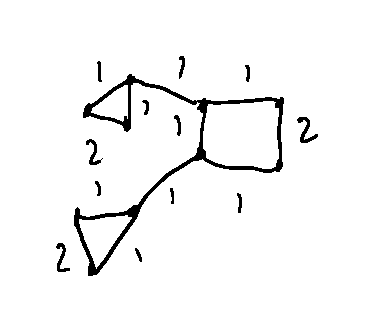
\includegraphics[width=.7\textwidth]{i1.pdf} In this case, $c=3$.
                \paragraph{Example 7}
                $G=(V,E)$ undirected graph degree of every vertex is
                $10$. Suppose to every vertex $v \in V$ a positive integer
                $a_v$ is assigned.
                \\ If $\sum_{v\in V}a_v = 5$ then what is $\sum_{u\in V}
                \sum_{\substack{w\in V:\\ uw\in E}} a_w = ? =\sum_{w \in
                  V}10a_w = 10 \times 5 =50$. Each $a_w$
                appears in the sum $10$ times since the degree of each
                vertex is $10$.
           \subsection{Topics Covered}
                The following are the topics we will be covering in
                this course:
                \begin{itemize}
                \item Network flows (More of like a practice topic for
                  what we'll be seeing in the course, will use the
                  algorithm to solve this problem for seemingly
                  unrelated problems. We'll be doing this a lot in the
                  course, called reduction, where we reduce solving
                  one problem to another problem.)
                \item Linear Programming (Bunch of constraints and
                  want to optimize a linear function). This will be
                  one of the most important concepts we learn in this
                  course.
                \item Midterm
                \item Linear Programming again
                \item NP-Completeness (no good algorithms for problems
                  that seem very basic, useful skill to have even if
                  you aren't a theoretician)
                \item Approximation algorithms (settling for the next
                  best thing for NP-Complete problems, might be able
                  to find an algorithm that approximates things, not
                  exactly optimal, but some sort of factor of how good
                  the approximation is; lots of research happening in
                  this area, better and better approximations). Will
                  use a lot of linear programming here.
                \item Randomized algorithms (randomness can actually
                  help us; probability theory/knowledge of random
                  variables may help a little bit here, but this is
                  the last stretch of the course and not very essential)
                \end{itemize}
         \subsection{Network Flows \\ Max Flow Problem}
            Very important, used in things like game theory.
            \underline{Def}: A flow is a \underline{directed} graph
            $G=(V,E)$ such that:
            \begin{enumerate}
            \item Every edge $e$ has a capacity $c_e \geq 0$.
            \item There is a source $s \in V$.
            \item There is a sink $t \in V$ such that $t\neq s$.
            \end{enumerate}
            \paragraph{Example}~\\
                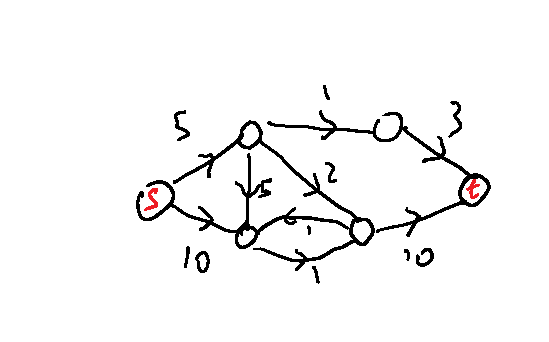
\includegraphics[width=.7\linewidth]{i2.pdf}
            \paragraph{Remark}: For the sake of convenience we make
            the following assumptions.
            \begin{enumerate}
            \item No edge enters the source.
            \item No edge leaves the sink.
            \item All capacities are integers.
            \item There is at least one edge incident to every vertex.
            \end{enumerate}
            \underline{Def}: [flow] A flow is a function $f:E
            \rightarrow \mathbb{R}^+$ such that: (Note that :$\mathbb{R}^+ = \{X \in
            \mathbb{R} | x \geq 0\}$)
            \begin{enumerate}[(i)]
            \item \text{[capacity]} $\forall e \in E, 0 \leq f(e) \leq
              c_e$ (flow cannot be negative nor can it exceed
              capacity)
            \item \text{[conservation]} For every node $u$ other than
              source and sink the amount of flow that goes into $u=$
              the amount of flow that leaves $u$. Formally:
              $$\forall u \in V\setminus\{s,t\} \underbrace{\sum_{vu\in E}f(uv)}_{f^{\text{in}}(u)} = \underbrace{\sum_{uw\in E}f(uw)}_{f^{\text{out}}(u)}$$
            \end{enumerate}
            \paragraph{Example}~\\
                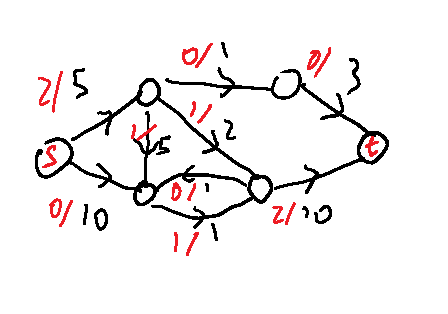
\includegraphics[width=.7\linewidth]{i3.pdf}
            \\ \underline{Def}: $Val(f) = \sum_{su\in E} f(su) =
            f^{\text{out}}(s)$
            \\\noindent\rule{\textwidth}{0.5pt}
            Max Flow Problem: Given a flow network find a flow with
            largest possible value.
    \section{01/10/18}
        \subsection{Max Flow Problem (Continued)}
        Recall: we want to process a flow network, essentially a
        directed graph with a source and a sink.
        \paragraph{A flow network}~\\
        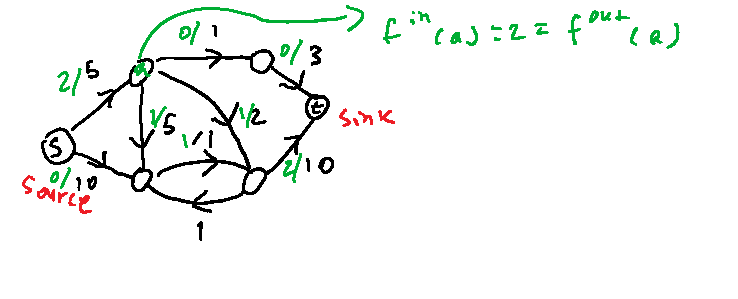
\includegraphics[width=.7\textwidth]{i4.pdf}
        \\ \rule{\textwidth}{0.5pt}
        $val(f)=f^{out}(s)$
        \\ Max Flow Problem: Given a flow network find the maximum
        value of the flow. $2$ is not the optimal value of the
        example. We could change it to:
        \\ 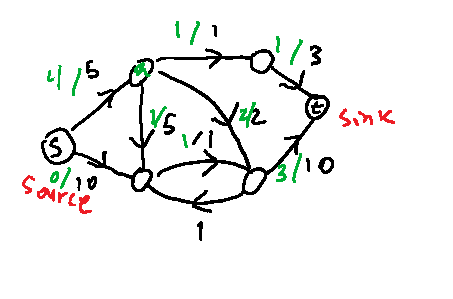
\includegraphics[width=.7\textwidth]{i5.pdf}
        \paragraph{Ford-Fulkerson Algorithm}
        Try to find $s-t$ paths that have not used their capacity and
        push more flow through them. There is a subtlety here
        though, we may run into trouble, like in the following example:
        \\ 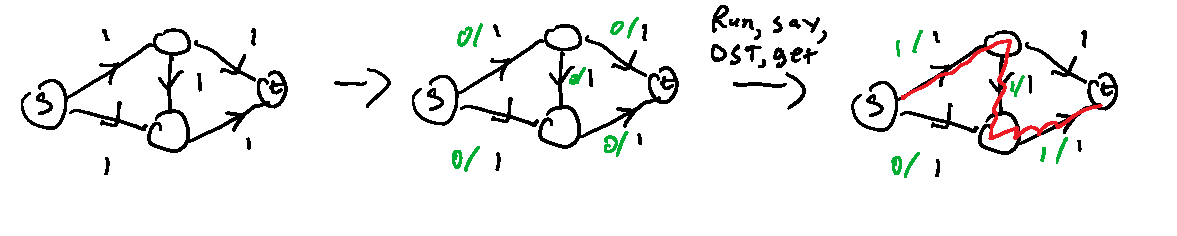
\includegraphics[width=\textwidth]{i6.pdf}
        \\ Now we are stuck. This is \textbf{not optimal}. The
        following is:
        \\ 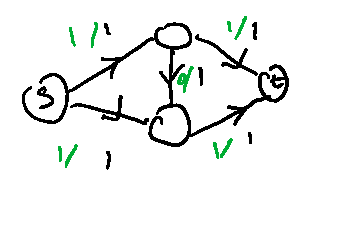
\includegraphics[width=.3\textwidth]{i7.pdf}
        \\ So we must change or else this algorithm won't work. We
        don't want to go back and change the first step, even though
        we are stuck. There is a way that we can change things. Say we
        try to add one more unit of flow:
        \\ 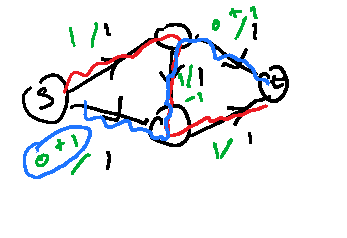
\includegraphics[width=.3\textwidth]{i8.pdf}
        \\ Essentially, the flow we added ``cancels'' the edge in the
        middle and makes it go back. Formally:
        \begin{enumerate}
        \item Start from the all zero flow.
        \item Find a ``path'' (not a real path since we can also
          reverse directions) from $s-t$ such that the edges that are
          in the forward direction have \textbf{unused capacity} (not
          saturated) and the backward edges have \textbf{strictly positive}
          flow on them. Add one unit to forward edges and subtract one
          unit from backwards edges. Repeat this step until we cannot
          find any more paths.
        \end{enumerate}
        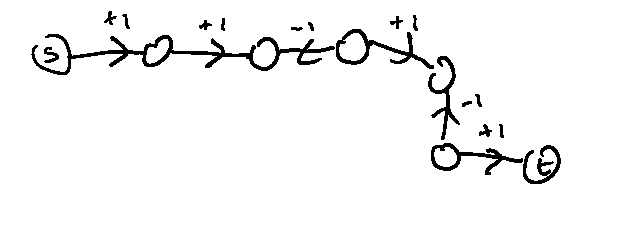
\includegraphics[width=.5\textwidth]{i9.pdf}
        \\ How do we implement this?
        \paragraph{Def} [Residual graph] Given a flow network
        $(G,s,t,\{c_e\})$ and an flow $f$ on $G$, the residual graph
        $G_f$ is as follows (we are already in the middle of the
        algorithm and this graph will tell us which edges are usable):
        \begin{enumerate}
        \item Nodes are the same as $G$.
        \item For every edge $uv \in G$ with $f(uv)<c_{uv}$ (flow
          strictly smaller than capacity), add the edge $uv$ with
          residual capacity $\mathbf{c_{uv}-f(uv)}$ to $G_f$.
        \item For every edge $uv \in G$ with $f(uv)>0$ add the
          opposite edge $\underline{vu}$ with residual capacity $f(uv)$.
        \end{enumerate}
        \rule{\textwidth}{0.5 pt}
        \paragraph{Example} ~ \\
        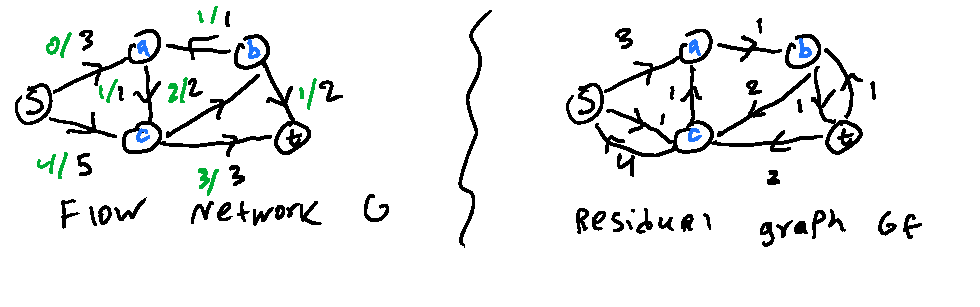
\includegraphics[width=\textwidth]{i10.pdf}
        \\ How do we use the residual graph? Just run a DFS on $G_f$
        to find an $s-t$ path and use it to modify the original flow,
        like so:
        \\ 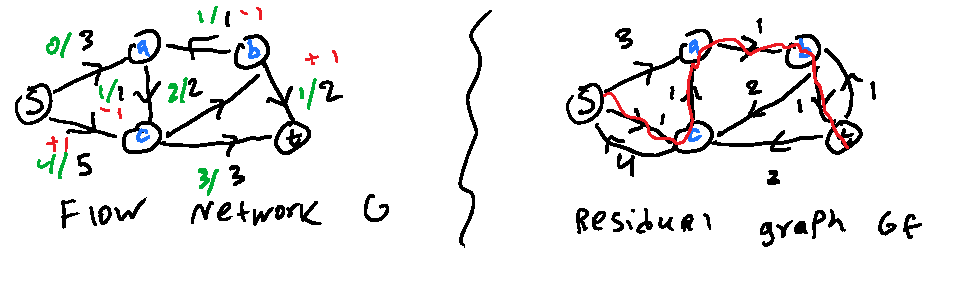
\includegraphics[width=\textwidth]{i11.pdf}
        \paragraph{Pseudocode for Ford-Fulkerson}
        \begin{algorithmic}
          \State Initially set $f(e)=0, \forall e \in E$
          \State Construct $G_f$
          \While{there is an $s-t$-path $P$ in $G_f$}
            \State $f' \gets$Augment$(f,p)$, where Augment means
            increase the flow using path $P$
            \State update $f \gets f'$
            \State update $G_f$
         \EndWhile
        \end{algorithmic}
        How many units of flow can we push if we find the following
        path in $G_f$?
        \\ 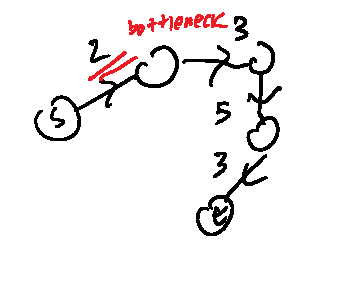
\includegraphics[width=.7\textwidth]{i12.pdf}
        \\ The smallest weight, the bottleneck.
        \begin{algorithmic}
          \State Augment$(f,P)$
          \State Find the bottleneck of $P$, which is the smallest
          residual capacity on $P$.
          \State For forward edges we add this number to their flow.
          \State For backward edges we subtract.
        \end{algorithmic}
        \paragraph{Example}~
        \\ 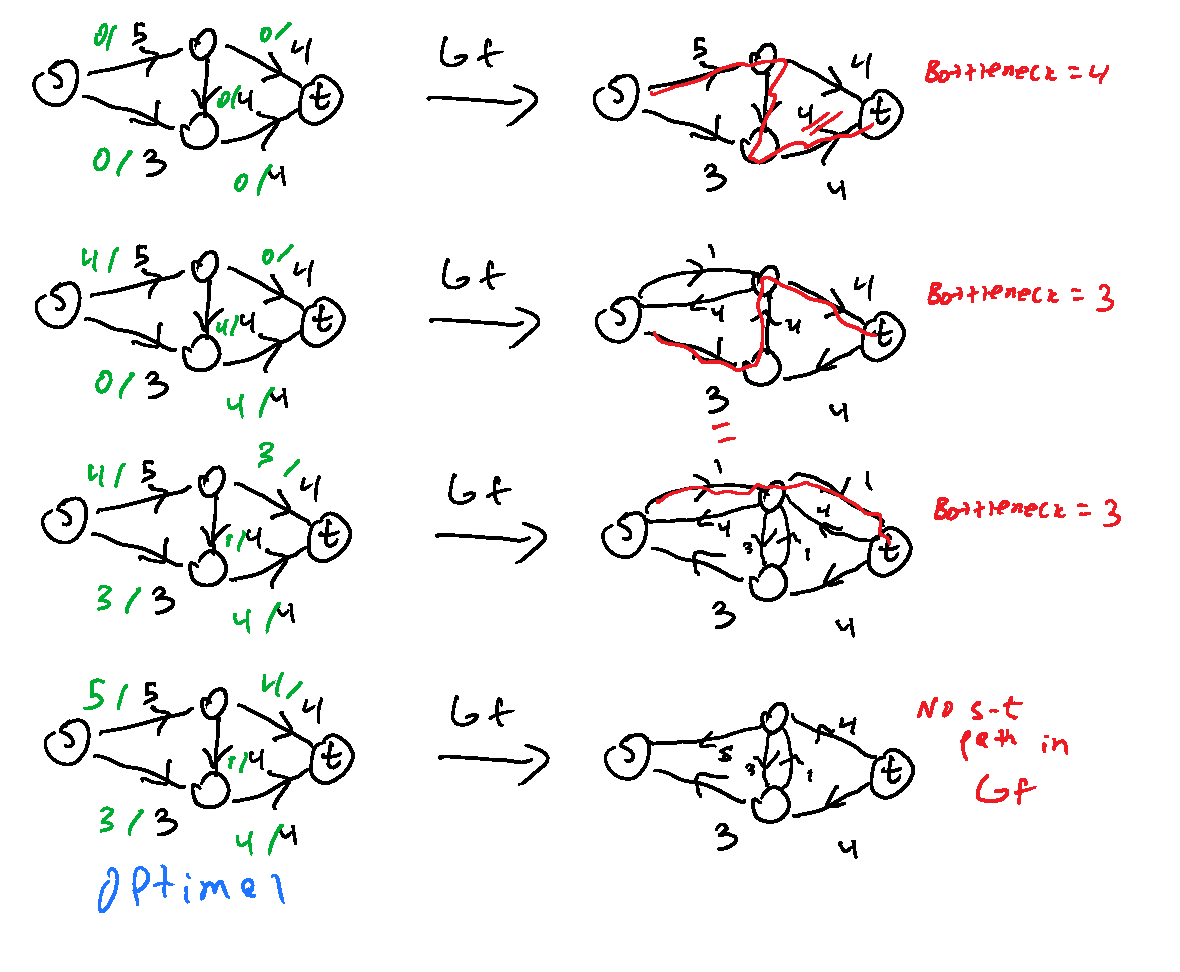
\includegraphics[width=\textwidth]{i13.pdf}
        \paragraph{Claim} FF always returns a valid flow (proof of
        correctness).
        \paragraph{Proof} Residual capacities are chosen so that
        updating with Augment$(f,P)$ will never assign a number to an
        edge that is larger than its capacity or smaller than
        $0$. $\implies$ capacity condition is satisfied throughout the
        algorithm.
        \paragraph{Conservation Condition} $f^{in}(v)=f^{out}(v)$
        \\ 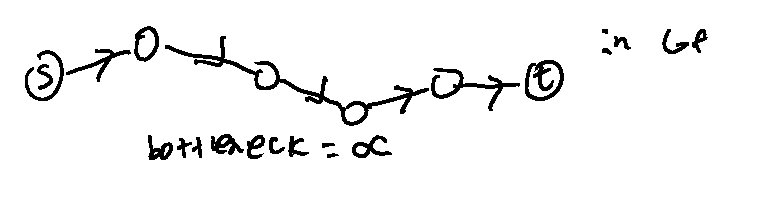
\includegraphics[width=.7\textwidth]{i14.pdf}
        \\ In G:
        \begin{itemize}
        \item Case 1:
        \\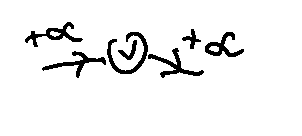
\includegraphics[width=.3\textwidth]{i15.pdf}
          \begin{align*}
            f^{in} \gets f^{in} + \alpha
            \\ f^{out} \gets f^{out} + \alpha
          \end{align*}
          Still the same.
        \item Case 2:
        \\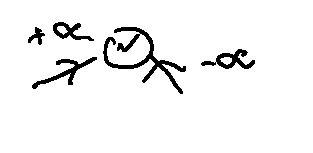
\includegraphics[width=.3\textwidth]{i16.pdf}
          \begin{align*}
            f^{in} \gets f^{in} + \alpha - \alpha
            \\ f^{out} \gets f^{out}
          \end{align*}
          Nothing changed.
        \item Case 3:
        \\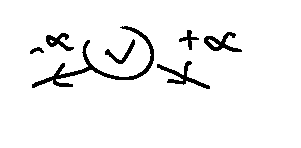
\includegraphics[width=.3\textwidth]{i17.pdf}
          \begin{align*}
            f^{in} \gets f^{in}
            \\ f^{out} \gets f^{out}-\alpha+\alpha
          \end{align*}
          Still equal.
        \item Case 4:
        \\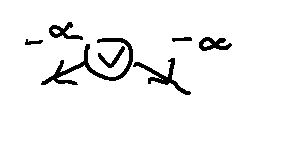
\includegraphics[width=.3\textwidth]{i18.pdf}
          \begin{align*}
            f^{in} \gets f^{in} - \alpha
            \\ f^{out}\gets f^{out} - \alpha
          \end{align*}
          Equal.
        \end{itemize}
        In all cases $f^{in}(v)$ remains equal to $f^{out}(v)$. So we
        have shown that the flow remains valid, but we still don't
        know if it gives us the optimal solution or not.
        \paragraph{Claim} The algorithm terminates.
        \paragraph{Proof} At every iteration, the flow increases by at
        least $1$ unit. It can never exceed the total sum of all the
        capacities, so it has to terminate.
        \paragraph{Running Time} Let $K$ be the largest capacity, $n$
        the number of vertices, $m$ the number of edges. There are at
        most $Km$ iterations. Finding an $s-t$-path:
        $O(m+n)$ (each iteration requires a DFS in the residual graph
        and an update). Augmenting: $(n)$.
        \\ Since we assumed every vertex is adjacent to at least one
        edge $\frac{n}{2}\leq m$ (with this assumption we can just
        talk about $m$). This makes the DFS $O(m)$.
        \\ The total running time:
        $$O(K \times m \times m) = O(Km^2)$$
        Unfortunately not that great if $K$ is a large number. We'll
        try to improve this a little bit later.
        \rule{\textwidth}{0.5pt}
        \subsection{Cuts}
        \paragraph{Def} A cut ($s-t$-cut) in a flow network is a
        partition $(A,B)$ of the vertices such that $s \in A, t\in B$.
        \paragraph{Def} Capacity of this cut is the sum of the
        capacities and edges going from $A$ to $B$.
        \\ 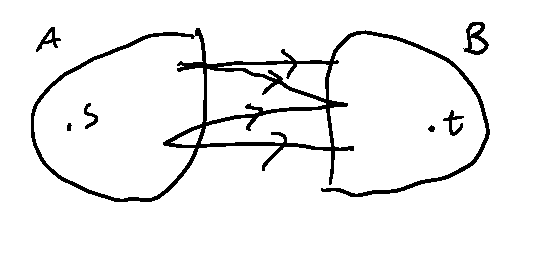
\includegraphics[width=.7\textwidth]{i19.pdf}
        $$cap(A,B)=\sum_{\substack{uv\in E \\ u \in A \\ v \in B}} c_{uv}$$
        \paragraph{Example}
        ~\\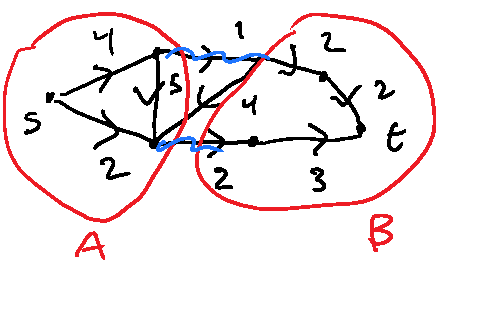
\includegraphics[width=.7\textwidth]{i20.pdf}
        \\ The capacity here is $3$. We see that we can't pass more
        weight from $A$ to $B$, i.e. cuts intuitively tell us
        something about the max flow.
        \\ How many cuts are in this network?
        \\ 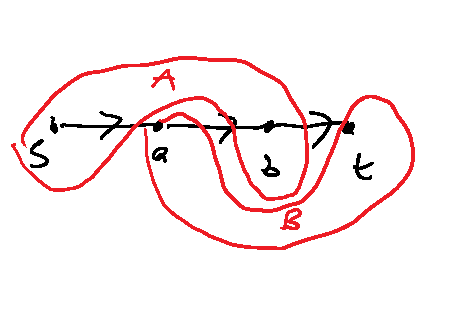
\includegraphics[width=.7\textwidth]{i21.pdf}
        \\ $4$. There's no geometry in cuts, the only restriction is
        that $s$ is in $A$ and $t$ is in $B$, doesn't matter how
        network is drawn.
        \\ A network with $n$ vertices has $2^{n-2}$
        $(s,t)$-cuts. ($n-2$ vertices each with two choices: $2\times
        2 \times \ldots \times 2=2^{n-2}$)
    \section{01/15/18}
        \paragraph{Recall} \textbf{Cut:} Partition of the vertices
        into two parts $A,B$ such that $s\in A, t \in B$.
        \\ 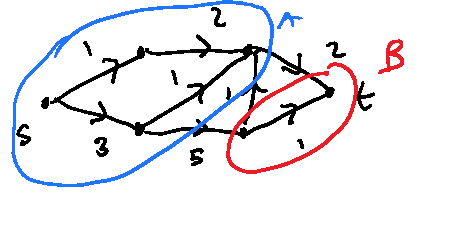
\includegraphics[width=.7\textwidth]{i22.pdf}
        In this example, the capacity is $5+2$
        $$Cap(A,B) = \sum_{\substack{uv \in E \\ u \in A \\ v \in B}}
        C_{uv}$$
        These capacities give us an upper bound on the maximum flow,
        but we have to prove this, intuition isn't enough. So how do
        we prove this?
        \\ \rule{\textwidth}{0.5 pt}
        \paragraph{Recall} For a flow $f:E \to \mathbb{R}^+$,
        $$val(f) = \sum_{su\in E} f(su)$$
        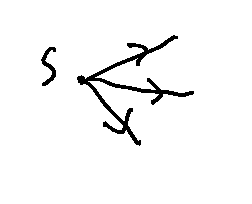
\includegraphics[width=.7\textwidth]{i23.pdf}
        Why do we define it this way? Why not talk about the flow
        going into the sink?
        \\ 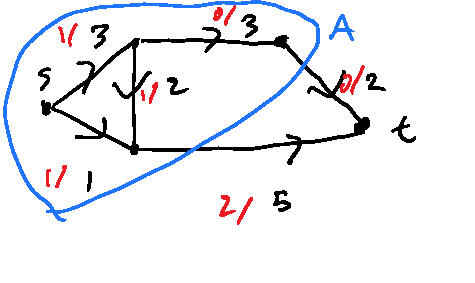
\includegraphics[width=.7\textwidth]{i24.pdf}
        In this example we see that $val=1+1=2$. We can also define a
        flow going into $t$. In this case it would also be $2$. Are
        they equal? Our intuition says yes, because none of the
        intermediate nodes are adding or absorbing flow.
        \\ \rule{\textwidth}{0.5pt}
        \paragraph{Claim} For any $s-t$-cut $(A,B)$, 
        $$val(f) = f^{out}(A) - f^{in}(A) = \sum_{\substack{uv \in E\\ u
            \in A \\ v \in B}}f(uv) - \sum_{\substack{uv \in E \\ u \in B
            \\ v \in A}} f(uv)$$
        In the example above, $f^{out}(A) = 1+1+0, f^{in}(A)=0$.
        \\ 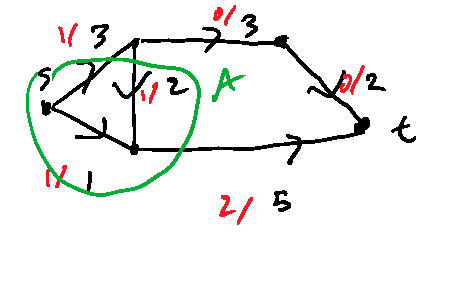
\includegraphics[width=.7\textwidth]{i25.pdf}
        \begin{flalign*}
          f^{out}(A)&=1+2, f^{in}(A)=1
          \\ val(f)&=\sum_{su\in E}f(su)=f^{out}(s) &
          \\ val(f) & = \sum_{u \in A}f^{out}(u)-f^{in}(u)
        \end{flalign*}
        $f^{out}-f^{in}$ is always $0$, unless $u$ is $s$ or $t$, but
        $t\notin A$.
        \begin{flalign*}
          \sum_{u \in A} \left( \left(\sum_{uv \in E}f(uw)\right) - \left(\sum_{vu \in E}f(vu)\right) \right)
        \end{flalign*}
        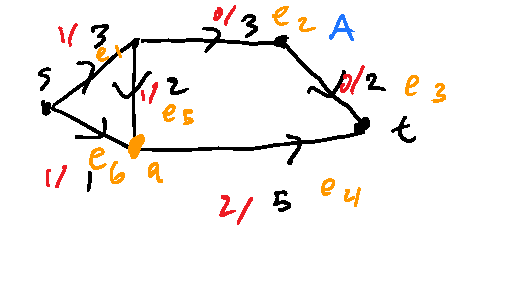
\includegraphics[width=.7\textwidth]{i26.pdf}
        \begin{flalign*}
          f^{out}(s) & = f(e_1)+f(e_6) &
          \\ f^{in}(s)&=0
          \\ f^{out}(a)&=f(e_4)
          \\ f^{in}(a) &= f(e_6)+f(e_5)
          \\
          \\ \left(f(e_1)+f(e_6) - 0\right) + \left(f(e_4)-f(e_6)-f(e_5)\right) & = \underbrace{f(e_1) + f(e_4)}_{f^{out}(a)}-\underbrace{f(e_5)}_{f^{in}(a)}
        \end{flalign*}
        Why did this come out to $f^{out}-f^{in}$? 
        \\ Looking back at the double sum above: If $e$ is an edge
        with both endpoints in $B \implies f(e)$ is not in the sum
        (since each term has at least one vertex in $A$). What if $e$
        has both endpoints in $A$? It will appear in the positive and
        negative sums, so they will cancel out, just like $e_6$ in our
        example.
        \paragraph{Observations}~
        \\ 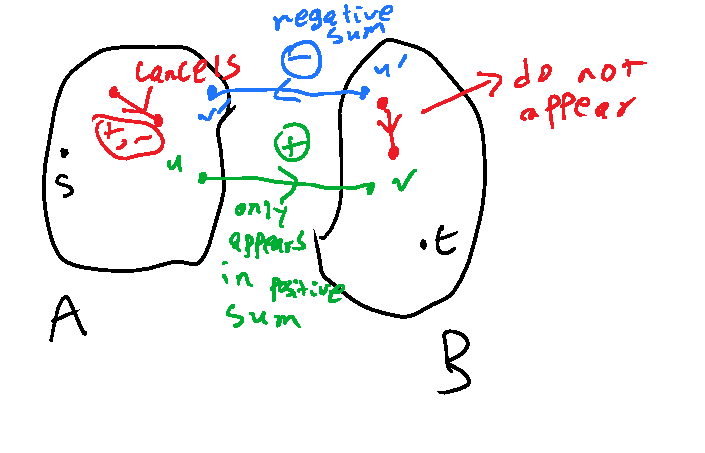
\includegraphics[width=.7\textwidth]{i27.pdf} Because of
        some cancellations here, we can simplify the sum:
        \begin{flalign*}
          \sum_{u \in A} \left(\sum_{uw \in E}f(uw) - \sum_{vu \in E}f(vu)\right)
          \\ = \sum_{\substack{uv \in E \\ u \in A \\ v \in B}}f(uv) - \sum_{\substack{uv \in E\\u \in B \\ v \in A}} f(uv) = f^{out}(A) - f^{in}(A)
        \end{flalign*}
        This concludes the proof of the claim. \hfill $\square$
        \\ Now why does $val(f) = f^{in}(t)$? Take the cut with
        $B=\{t\}$.
        \\ 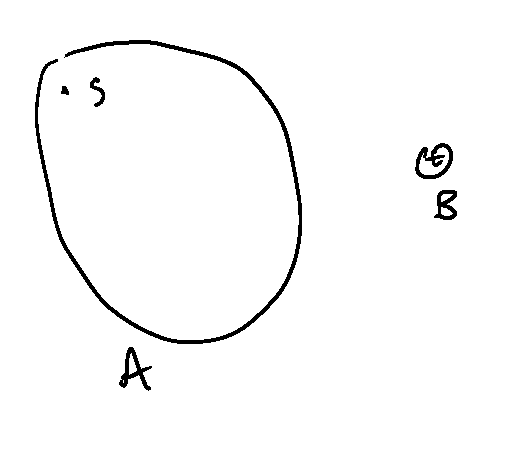
\includegraphics[width=.4\textwidth]{i28.pdf}
        Then by the claim:
        $$val(f) = \underbrace{f^{out}(A)}_{f^{in}(t)} -
        \underbrace{f^{in}(A)}_0$$
        \paragraph{Corollary to this claim} Let $(A,B)$ be a cut, $f$
        be a flow. Then $val(f)\leq cap(A,B)$. i.e. the flow cannot
        exceed the capacity of the cut, any arbitrary cut puts an
        upper bound on the flow. How can we prove this using the
        previous claim?
        \paragraph{Proof}
        \begin{flalign*}
          val(f) & = f^{out}(A) - f^{in}(A) \leq f^{out}(A) = \sum_{\substack{u \in A \\ v \in B \\ uv \in E}}f(uv) \leq \sum_{\substack{u \in A \\ v \in B \\ uv \in E}}C_{uv} = cap(A,B)&
        \end{flalign*}
        In other words, the flow of each edge is bounded by the
        capacity of each edge, but then this is just the definition of
        the capacity of a cut. Now why is this corollary useful? Let's
        look at an example.
        \paragraph{Example} ~
        \\ 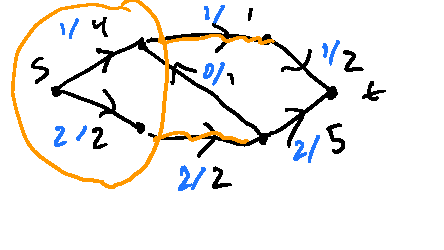
\includegraphics[width = 0.7\textwidth]{i29.pdf}
        $cap(A,B)=1+2 = 3$ and $val=3 \implies$ max flow $= 3$. So if
        we get a flow and are asked if this is the max flow or not,
        either we find a flow with a better value to disprove it, or
        find a cut such that the capacity is the same as the flow, to
        prove that we can't do any better than that.
        \paragraph{Proof of the fact that Ford-Fulkerson finds the max
          flow} Recall:
        \begin{algorithmic}
          \State{FF: start with $f = 0$}
          \While{$s-t$ path $p$ in $G_f$}
            \State{Augment$(f,p)$}
            \State{update $G_f$}
          \EndWhile
        \end{algorithmic}
        Consider the point where Ford-Fulkerson terminates. Let $A^*$
        be the set of the vertices that can be reached from $S$ in
        the residual graph. Why is this a valid cut? Because at
        termination, there are no more $s-t$ paths, so $t \notin A^*$.
        \\ 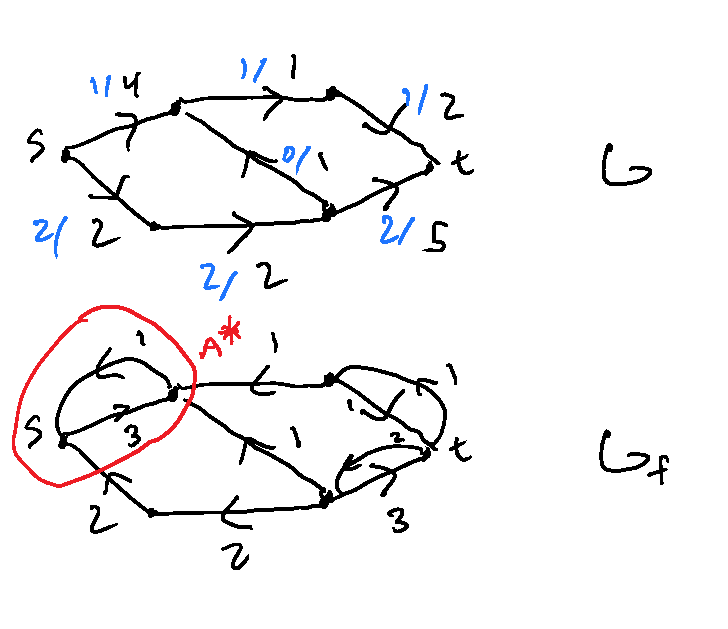
\includegraphics[width=0.7\textwidth]{i30.pdf}
        \\ 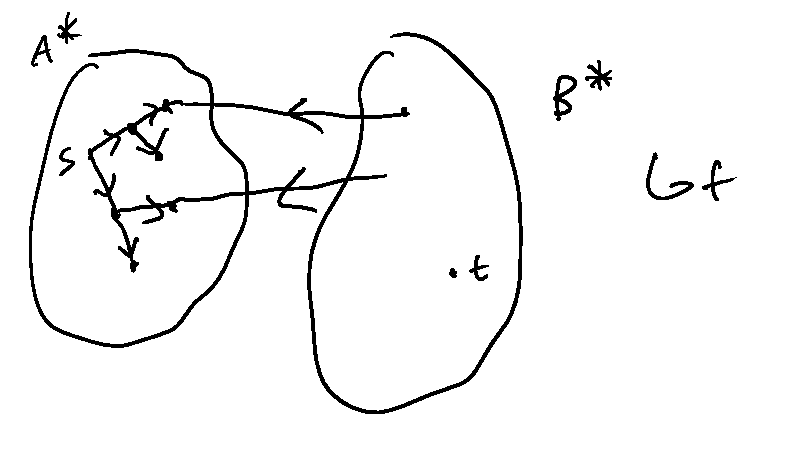
\includegraphics[width=0.7\textwidth]{i31.pdf}
        There are no edges in $G_f$ from $A^*$ to $B^*$, or else the
        endpoint vertex in $B^*$ would be in $A^*$, because $A^*$
        consists of all the vertices we can reach from $s$. Thus:
        if $uv$ is an edge in the original network with $u \in A^*, v
        \in B^*$
        \\ 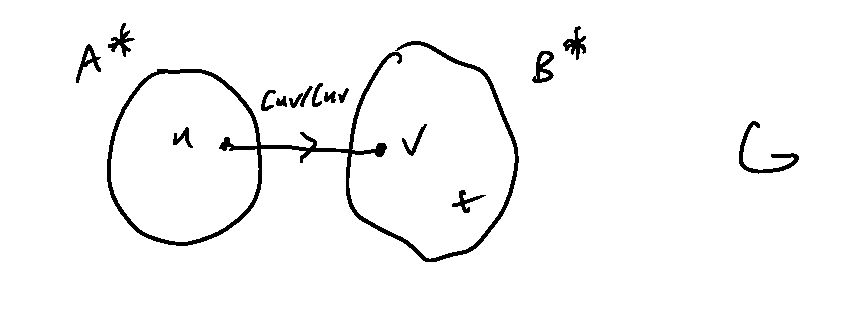
\includegraphics[width=0.7\textwidth]{i32.pdf}
        $f(uv) = C_{uv}$, or else the edge $uv$ would be in $G_f$.
        \\ 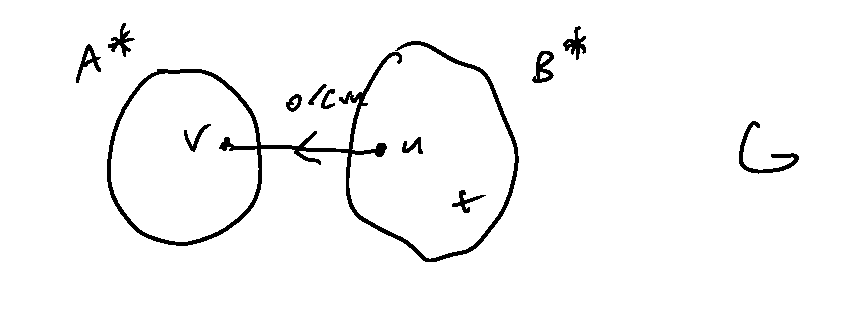
\includegraphics[width=0.7\textwidth]{i33.pdf}
        $f(uv) = 0$, otherwise $vu$ would be in $G_f$.
        Thus:
        \begin{flalign*}
          f^{in}(A^*) & = 0
          \\ f^{out}(A^*) & = \sum_{\substack{u \in A^* \\ v \in B^* \\ uv \in E}} C_{uv} = cap(A^*,B^*)
        \end{flalign*}
        Therefore,
        $$val(f) = f^{out}(A^*)-f^{in}(A^*) = cap(A^*,B^*)$$
        So we showed that Ford-Fulkerson finds the cut that maximizes
        the flow, i.e. Ford-Fulkerson gives us the optimal
        solution. We have:
        \begin{flalign*}
          max\hbox{-}flow \leq cap(A^*,B^*) = val(f) \implies val(f) = max\hbox{-}flow
        \end{flalign*}
        % \rule{\textwidth}{0.5pt}
        % We showed that Ford-Fulkerson finds max flow. That is, when it
        % terminates, $val(f) = max\hbox{-}flow$
        % \\ \rule{\textwidth}{0.5pt}
        \paragraph{Problem} Given a flow network how can we find a
        min\hbox{-}cut? Run Ford-Fulkerson and output $(A^*, B^*)$.
        \begin{flalign*}
          \underbrace{val(f)}_{\text{any flow }f} & \leq max\hbox{-}flow \leq min\hbox{-}cut \leq cap(A^*,B^*)
        \end{flalign*}
        When we run Ford-Fulkerson we find $f$ with
        $val(f)=cap(A^*,B^*)$
        $$\implies val(f) = \mathbf{max\hbox{-}flow = min\hbox{-}cut} =
        cap(A^*,B*)$$
        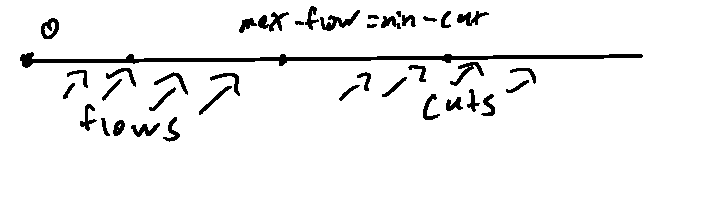
\includegraphics[width=0.7\textwidth]{i34.pdf}
        \paragraph{Thm} For any flow network:
        $$max\hbox{-}flow = min\hbox{-}cut$$
        \section{01/17/18}
        \paragraph{Recall}
        \begin{itemize}
        \item Ford-Fulkerson finds the max flow. 
        \item $max\hbox{-}flow=min\hbox{-}cut$. Kind of unexpected/unintuitive that
          they'd be equal. It's pretty intuitive that $min\hbox{-}cut$ is an
          upper bound, but it's surprising that they are equal.
        \item Ford-Fulkerson runs in $O(m^2K)$, where $m$ is the
          number of edges, $K$ is the
          largest capacity of an edge. Can be quite slow if the
          largest capacity is big.
        \item $val(f) =f^{out}(s)=f^{in}(t)=f^{out}(A)-f^{in}(A)$ for
          all cuts $(A,B)$
        \item Ford-Fulkerson can be used to find $min\hbox{-}cut$.
          \\ 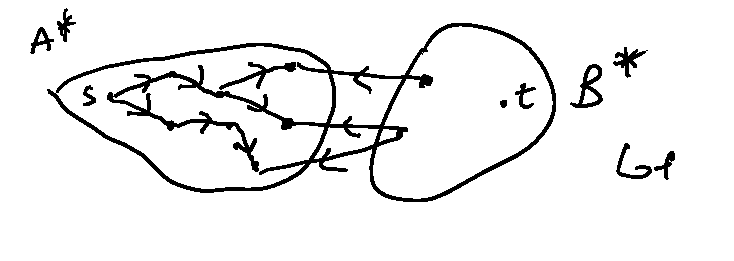
\includegraphics[width=.9\textwidth]{i35.pdf}
          Can't reach $t$ from $s$ at the end of the algorithm in the
          residual graph.
        \end{itemize}
        \paragraph{Question} (Recall all capacities are integers) Is
        it possible to have a $max\hbox{-}flow$ that assigns non-integer
        values to some of the edges? (Remember that the flow function
        is defined as $f:E \to \mathbb{R}^+$) Yes, it is possible:
        \\ 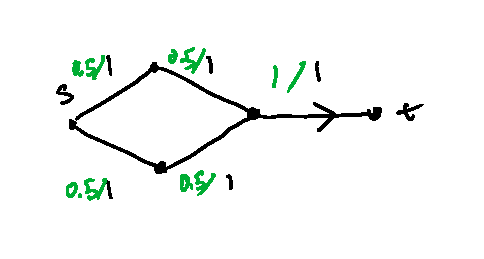
\includegraphics[width=.9\textwidth]{i36.pdf}
        \paragraph{Question} Is there always an all integer
        $max\hbox{-}flow$? Yes because Ford-Fulkerson always outputs integer
        valued flows and we know that it finds $max\hbox{-}flow$. i.e. there
        is at least one all integer $max\hbox{-}flow$, the one that can be
        found by Ford-Fulkerson and we already proved that it gives
        $max\hbox{-}flow$. If you try to prove this directly, it seems very
        hard unless you come up with something like Ford-Fulkerson. So
        we have obtained many important consequences and applications
        from analyzing Ford-Fulkerson.
        \paragraph{Remark} The running time $O(m^2K)$ is not efficient
        when $K$ is a large number. Input size: $\Theta(m \log k)$,
        since we have $m$ edges each that require as much as $\log k$
        bits to write each number between $1-K$. (This is an
        exponential time algorithm)
        \\ 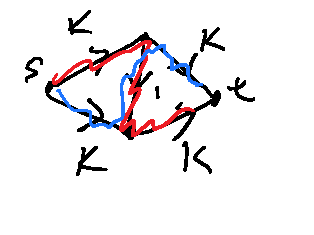
\includegraphics[width=.9\textwidth]{i37.pdf} Running
        Ford-Fulkerson on this graph would require $2^K$ path
        augmentations, alternating between the red and blue path. So
        we want to get rid of this and improve it.
        \subsection{A Faster Ford-Fulkerson}
        \paragraph{Possible Approaches}
        \begin{enumerate}
        \item Always pick the shortest path from $s$ to $t$. This will
          work and leads to an efficient (polytime) algorithm. We will
          not discuss it here. Pretty easy to implement too, just run
          a BFS instead of a DFS.
        \item Try to go with the paths that increase the flow by
          larger numbers. In the above example, we see that the red
          path only increases flow by $1$, instead of the top path
          that can increase it by $K$. This is called the Fattest Path
          approach, where we find an augmenting path with the largest
          bottleneck. However, there is a bit of a problem here,
          finding this path is a bit complicated and not fast. (There
          is a way to implement it by modifying Dijkstra's, but not so
          fast)
          \\ The problem with the first proposed solution is that it
          can't be analyzed easily (although it can be implemented
          easily), whereas the second solution can be analyzed easily
          but not easily implemented.
        \end{enumerate}
        We will do something similar:
        \paragraph{High level description}
        \begin{algorithmic}
          \State Initially set $\Delta = 2^{\lceil \log_2 k \rceil}$,
          that is $\Delta$ is the smallest power of $2$ that is at
          least $K$. (e.g. $K=13 \implies \Delta = 16, K=17 \implies
          \Delta = 32$)
          \While{\underline{there are augmenting paths with
            bottleneck$\geq\Delta$}} use them to augment the flow
          \State When we run out of these we set $\Delta \gets
          \frac{\Delta}{2}$
          \State If $\Delta=1$ here (when we want to decrease it) then stop.
          \EndWhile
        \end{algorithmic}
        How can we check the underlined condition, that there are
        augmenting paths with bottleneck greater than $\Delta$?
        \\ 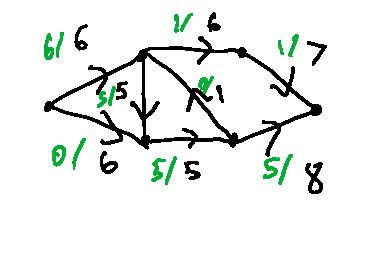
\includegraphics[width=.9\textwidth]{i38.pdf} with
        $\Delta=4$.
        \\In this case, when we build the residual graph we will
        exclude edges that have weight less than $4$. Let
        $G_f(\Delta)$ be the subgraph of $G_f$ consisting only of the
        edges with residual cap $\geq \Delta$. We just need to find an
        $s-t$ path in $G_f(\Delta)$.
        \\ 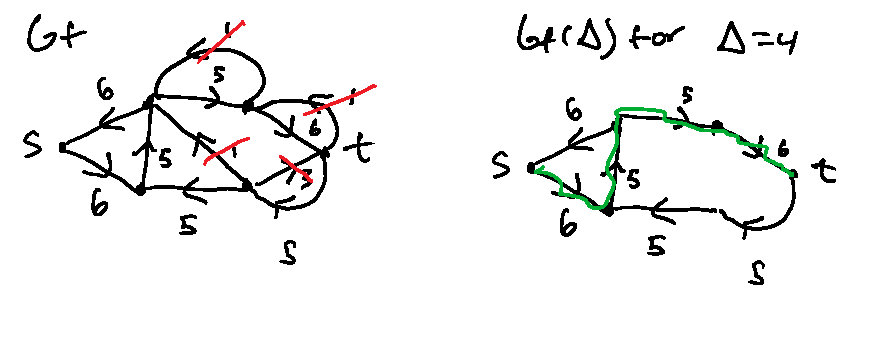
\includegraphics[width=.9\textwidth]{i39.pdf}
        \\ Here bottleneck$\geq \Delta$, we can increase the flow by
        $5$ here.
        \\ We call this scaling.
        \paragraph{Scaling Ford-Fulkerson}
        \begin{algorithmic}
          \State set $\Delta=2^{\lceil \log_2 k \rceil}$, where $K$ is
          the largest capacity.
          \State set $f=0$, construct $G_f$
          \While{$\Delta \geq 1$}
            \While{$\exists$ an $s-t$ path $P$ in $G_F(\Delta)$}
                \State{Augment$(f,p)$}
                \State{update $G_f$}
            \EndWhile
            \State $\Delta \gets \frac{\Delta}{2}$    
          \EndWhile
        \end{algorithmic}
        \paragraph{Running Time}
        \begin{itemize}
        \item Checking if there exists an $s-t$ path: $O(m)$
        \item Augmenting, $O(m)$
        \item Updating $G_f$, $O(m)$
        \end{itemize}
        So we need to understand the number of iterations.
        The outer loop has $\lceil \log_2 K \rceil$ iterations. The
        inner loop? (actually will be a bit of work to analyze this.)
        How many times in the $\Delta-phase$?
        \paragraph{Claim} Let $f$
        be the flow at the end of the $\Delta$-phase (when no $s-t$
        paths are in $G_f(\Delta)$). There is a cut $(A,B)$ such
        that $$max\hbox{-}flow \leq Cap(A,B) \leq val(f)+m\Delta$$
        \paragraph{Proof} Let $A$ be the set of all nodes that can be
        reached from $s$ in $G_f(\Delta)$ (very similar to $min\hbox{-}cuts$
        before)
        \\ 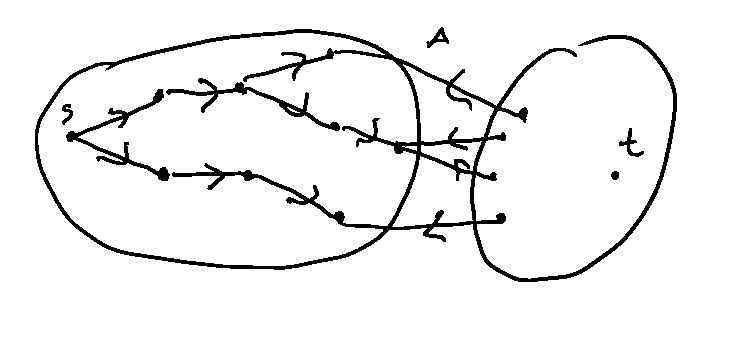
\includegraphics[width=.9\textwidth]{i40.pdf}
        \\ (No edge from $A$ to $B$ in $G_f(\Delta)$, otherwise $A$
        would have been extended further)
        \\ If $e$ is an edge from $A$ to $B$ in the original network:
        \\ 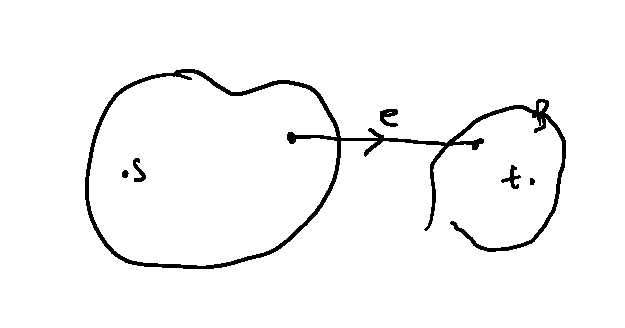
\includegraphics[width=.9\textwidth]{i41.pdf}
        \begin{align*}
          f(e) \geq c_e - \Delta
          \\ c_e - f(e) < \Delta
        \end{align*}
        If $e$ goes from $B$ to $A$:
        \\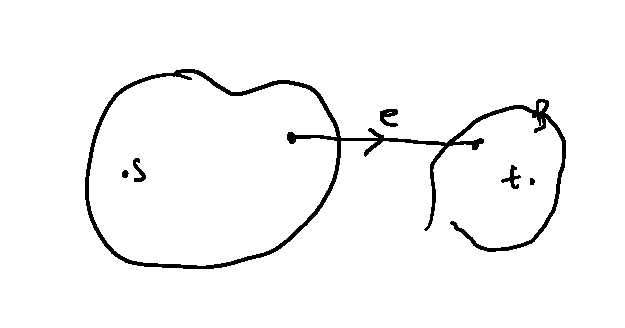
\includegraphics[width=.9\textwidth]{i41.pdf}
        \begin{align*}
          f(e) < \Delta
        \end{align*}
        Or else we could expand $A$.
        \begin{align*}
          val(f) & = f^{out}(A)-f^{in}(A) = \sum_{\substack{e \ from \\ A \ to \ B}} f(e)- \sum_{\substack{e \ from \\ B \ to \ A}}f(e)
          \\ & \geq \sum_{\substack{e \ from \\A \ to \ B}} (c_e - \Delta) - \sum_{\substack{e \ from \\ B \ to \ A}}\Delta = \sum_{\substack{e \ from \\ A \ to \ B}}c_e - \sum_{\substack{e \ from \\ A \ to \ B \\ or \ B \ to \ A}} \Delta
          \\ & = Cap(A,B) -m\Delta \implies val(f) \geq Cap(A,B)-m\delta 
        \end{align*}
        \hfill $\square$
        So we showed $$val(f) \geq Cap(A,B)-m\Delta \geq max\hbox{-}flow -
        m\Delta$$
        Let's look at the flow at the end of the previous phase.
        $$Val(f_{prev})\geq max\hbox{-}flow - 2\Delta m$$ (since we halved
        $\Delta$)
        \\ How many augmentations can we have in the $\Delta$-phase?
        %Every time you increase the $max\hbox{-}flow$, you are increasing it
        %by $\Delta$, and you cannot pass $2\Delta m$, so
        We can have at most $2m$ augmentations in this phase because each one
        increases the value by at least $\Delta$ and starting from
        $max\hbox{-}flow-2m\Delta$ we cannot go above $max\hbox{-}flow$. So the
        number of iterations of this is good as it only depends on
        $m$.
        \\ Back to the analysis, we figured out that the inner loop
        has $\leq 2m$ iterations. So the total running time is:
        \begin{align*}
          O(\log_2 K \times m \times m) = O(m^2 \log K)
        \end{align*}
        Instead of $O(m^2K)$ of the naive Ford-Fulkerson. This is a
        big improvement when $K$ is a huge number.
        \\ One thing is left: Why does this algorithm find the
        $max\hbox{-}flow$? Because when it terminates, $\Delta=1$ and it
        means there are no more augmenting $s-t$ paths in the residual
        graph.
        \paragraph{Remark} This is a special instance of
        Ford-Fulkerson $\implies$ it finds $max\hbox{-}flow$.
        \section{01/22/18}
        \paragraph{Recall}
        \begin{itemize}
        \item Ford Fulkerson finds max\hbox{-}flow $O(m^2K)$.
        \item \textbf{Scaling Ford Fulkerson} finds max\hbox{-}flow $O(m^2 \log K)$,
          $K=$largest capacity.
        \item $Max\hbox{-}flow=Min\hbox{-}cut$
        \item There is a $max\hbox{-}flow$ that assigns integer flows
          to all edges.
          \\ 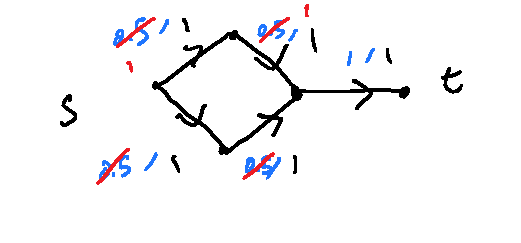
\includegraphics[width=.9\textwidth]{i42.pdf}
        \end{itemize}
        \paragraph{Bipartite Graph} is an undirected graph such that
        the vertices can be partitioned into two parts $X$ and $Y$
        such that all the edges are between $X$ and $Y$.
        \\ 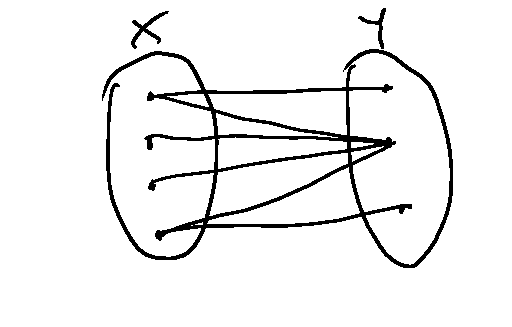
\includegraphics[width=.9\textwidth]{i43.pdf}
        \paragraph{Examples}Is this bipartite? Yes. We can check by
        just 2 coloring.
        \\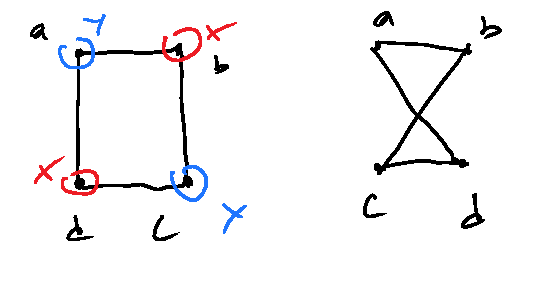
\includegraphics[width=.7\textwidth]{i44.pdf}
        \\ What about the Peterson graph? No.
        \\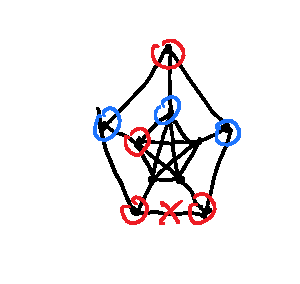
\includegraphics[width=.7\textwidth]{i45.pdf}
        We can just color it until we reach a contradiction.

        A graph is bipartite $\iff$ it does not have any odd
        cycles. Trivially a bipartite graph does not have an odd
        cycle: \\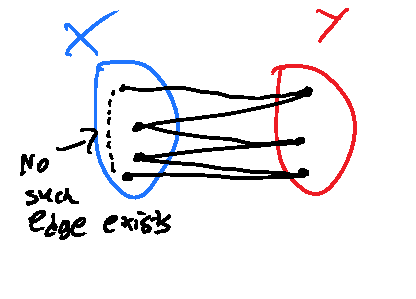
\includegraphics[width=.9\textwidth]{i46.pdf}
        \subsection{Largest Matching Problem}
        \paragraph{Def}A matching is a set of edges, no two of them
        share an endpoint.
        \paragraph{Def} A perfect matching is a matching that includes
        all vertices.
        \paragraph{Ex} The maximum matching of both of these graphs is
        $2$:
        \\ 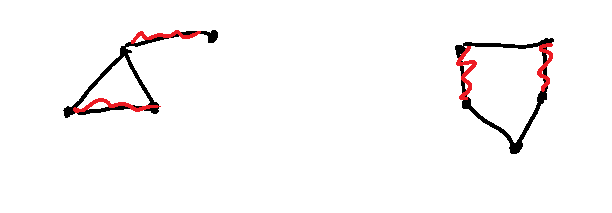
\includegraphics[width=.9\textwidth]{i47.pdf}
        \\ Note that there is nothing geometric about a matching, it
        does not matter how you draw the graph, the fact that the
        edges ``cross'' over each other does not matter, like here:
        \\ 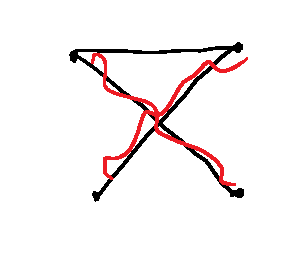
\includegraphics[width=.7\textwidth]{i48.pdf}
        \\ \noindent \rule{\textwidth}{0.5pt}
        Given a bipartite graph with parts $X$ and $Y$, how can we
        find the largest matching in $G$?
        \paragraph{Ex} Maximum matching here is $4$:
        \\ 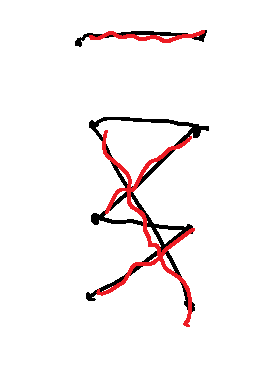
\includegraphics[width=.5\textwidth]{i49.pdf} Greedy
        algorithms won't work here, so how should we solve this?

        Why do we care about this problem? It has a very practical
        application, you can imagine it as a pairing of objects or
        something like pairing people with jobs, where every person
        has specific traits for certain jobs and we want to give as
        many people as possible a job, although each person can only
        have one.

        We want to use the max flow problem here. How will we do so?
        \paragraph{Solution} We construct a flow network in the
        following manner: 
        \begin{enumerate}
        \item We direct all the edges from $X$ to $Y$.
        \item We add two new vertices called $s$ and $t$.
        \item We put edges from $s$ to all vertices in $X$ and edges
          from all vertices in $Y$ to $t$.
        \item Assign capacity $1$ to all the edges.
        \end{enumerate}
        \includegraphics[width=.9\textwidth]{i50.pdf}
        \paragraph{Claim} Max flow in this network $=$ max matching in
        $G$.
        \paragraph{Proof} First we show max matching $(M)$ is at least
        max\hbox{-}flow.
        \\ \includegraphics[width=.9\textwidth]{i51.pdf}
        
        We assign a flow of $1$ to all edges in $M$ and $0$ to all
        other edges between $X$ and $Y$. For the edges starting from
        $s$ or ending at $t$, the ones that go to vertices in $M$ get
        a value of $1$ and the rest $0$.
        \\ \includegraphics[width=.9\textwidth]{i52.pdf}

        Why is this a valid flow? We aren't overloading capacities
        (only assigning $0$ or $1$) and we conserve flow going out of
        $s$ to flow going into $t$, since every edge in $M$ has $1$
        vertex with an edge coming from $s$ and one with an edge going to $t$. The value of this
        flow is $|M|$. This is because there are $|M|$ vertices in $X$
        involved in $M$ and we assign $1$ to the edges from $s$ to
        those vertices.
        \\ \noindent \rule{\textwidth}{0.5pt}
        Now we want to do the opposite, convert the max\hbox{-}flow to
        a matching.

        Next we need to show that there is a matching of size
        max\hbox{-}flow (assuming all edges are assigned either $1$ or
        $0$ flow, making the existence of an integer value flow proved
        last class important).

        There is a max\hbox{-}flow with integer values. Thus all edges
        will have a flow of $0$ or $1$ (the capacities are all $1$).

        The edges between $X$ and $Y$ with $1$ unit of flow on them
        form a matching.
        \\ \includegraphics[width=.9\textwidth]{i53.pdf}

        To summarize, we showed
        $$|M| \leq max\hbox{-}flow$$ and $$max\hbox{-}flow =
        \text{some matching} \leq \text{max matching} = |M| \implies
        |M| = max\hbox{-}flow$$
        \paragraph{Remark} Note that in the above proof we could
        assign $\infty$ capacities (instead of $1$ to all) to edges
        between $X$ and $Y$.
        \\ \includegraphics[width=.9\textwidth]{i54.pdf}

        The incoming flow of all vertices in $X$ will be at most $1$
        so the edges between $X$ and $Y$ will never have any flow
        $>1$. This will be useful when considering $min\hbox{-}cut$,
        as it eliminates many cuts.

        We know $max\hbox{-}flow=min\hbox{-}cut$. What does this mean
        in this context? (matching)
        \paragraph{Def}A vertex cover is a set of vertices such that
        removing them will remove all the edges.
        \\ \includegraphics[width=.7\textwidth]{i55.pdf}

        Here, the red vertices form a vertex cover. How can we find
        the smallest vertex cover? If we want to think of this
        practically, we can think of the vertices as monitors such
        that we can monitor all the connections/roads.
        \paragraph{Thm} In every bipartite graph max matching $=$ min
        vertex cover.

        \paragraph{Remark} Note that if a graph has a matching of size
        $k$, then every vertex cover needs to pick at least one vertex
        from each of these $k$ edges and thus is of size $\geq k$.
        % Why can't the min vertex cover be strictly smaller? Well you
        % need at least as many vertices as the matching, or else you'll
        % leave out a pair of edges.
        \paragraph{Remark} The equality is not true in general graphs.
        \\ \includegraphics[width=.6\textwidth]{i56.pdf}
        Here the max matching is $1$ but the minimum vertex cover is
        $2$.
        \\ \includegraphics[width=.9\textwidth]{i57.pdf}
        Lets look at the min cut $(A,B)$ (it is not $\infty$, can
        easily show one that isn't). Some vertices of $A$ are in $X$
        ($A_1$), others are in $Y$ ($A_2$), etc.
        \\ \includegraphics[width=.9\textwidth]{i58.pdf}

        $A=\{s\}\cup A_1 \cup A_2, B=B_1 \cup B_2 \cup \{t\}$
        \\ \includegraphics[width=.9\textwidth]{i59.pdf}

        No edges from $A$ to $B$ with $\infty$ cap $\implies$ no edges
        from $A_1$ to $B_2$. How can we use this to make a minimum
        vertex cover?

        $B_1 \cup A_2$ is a vertex cover in $G$.
        \\ \includegraphics[width=.9\textwidth]{i60.pdf}

        The only edges that could remain are from $A_1$ to $B_2$, but
        we just showed that those couldn't exist (to continue next class).
        \section{01/24/18}
        \paragraph{Recall} Matching in Bipartite graphs.
        \\ \includegraphics[width=.9\textwidth]{i61.pdf}
        \\ Ford Fulkerson can be used to find the largest matching in
        a Bipartite graph.
        \\ \includegraphics[width=.9\textwidth]{i62.pdf}
        \paragraph{Vertex Cover} A set of vertices such that deleting
        them will remove all the edges.
        \\ \includegraphics[width=.9\textwidth]{i63.pdf}
        \paragraph{Thm} For every bipartite graph $G$ we have
        $$ \min\hbox{VC} = max\hbox{-}matching$$
        \paragraph{Pf} Consider a $min\hbox{-}cut$ $(A,B)$ in the
        constructed flow network.
        \\ \includegraphics[width=.9\textwidth]{i64.pdf}
        \\ $A=\{s\} \cup A_1 \cup A_2, B= \{t\} \cup B_1 \cup B_2$

        No edges from $A_1$ to $B_2$ as otherwise the capacity at the
        cut would be $\infty$. Thus $B_1 \cup A_2$ is a vertex cover
        in the original graph. Its size is $|B_1|+|A_2|$. On the other
        hand,
        $$Cap(A,B) = \sum_{\substack{\text{edges from} \\ s\text{ to }B_1}} c_{sv}
        + \sum_{\substack{\text{edges from} \\ A_2\text{ to }t}} c_{vt}= |B_1| + |A_2|$$
        We showed that there is a vertex cover $(B_1 \cup A_2)$ whose
        size is equal to $min\hbox{-}cut$ $(A,B)$ ($min\hbox{-}VC \leq
        min\hbox{-}cut$).

        Next we will show that
        $$min\hbox{-}cut \leq min\hbox{-}vc = |S| = |S_1| + |S_2|$$
        Let $S$ be the smallest vertex cover.
        \\ \includegraphics[width=.9\textwidth]{i65.pdf}

        $S = S_1 \cup S_2, B=A^c$
        
        Let $A=(X-S_1)\cup S_2 \cup \{s\}$. $Cap(A,B)=
        \underbrace{|S_1|}_{\text{edges from $S$ to $S_1$}} +
        \underbrace{|S_2|}_{\text{edges from $S_2$ to $t$}}$

        We conclude $$Max\hbox{-} flow = Min\hbox{-}Cut = Min\hbox{-}Vc = Max\hbox{-}Matching$$

        \paragraph{Thm} (K\"onig) In a bipartite graph $Max\hbox{-}Matching =
        Min\hbox{-}Cut$
        \subsection{Disjoint Paths in directed graphs}
        Input: A directed graph and two distinct nodes are marked as
        $\underline{s}$ and $\underline{t}$.
        \\ Goal: Find the maximum number of edge-disjoint paths from
        $s$ to $t$.
        \paragraph{Ex}~
        \\ \includegraphics[width=.9\textwidth]{i67.pdf}

        Could we just use BFS or DFS to find an s-t path? No, it
        might chose the wrong edges like in this example:
        \\ \includegraphics[width=.9\textwidth]{i68.pdf}

        What if we chose the shortest path? That would also be
        problematic:
        \\ \includegraphics[width=.9\textwidth]{i69.pdf}

        How do we solve this then? We assign capacity $1$ to all the
        edges and run the Ford Fulkerson algorithm (note that we
        explicitly specify using Ford Fulkerson so we get integer
        values, not just max-flow).
        \paragraph{Ex} ~
        \\ \includegraphics[width=.9\textwidth]{i69.pdf}
        So the max-flow here is $3$. How do we show there are $3$ edge-disjoint paths?

        We solved the $max\hbox{-}flow$ using Ford Fulkerson and let
        $k$ be the value of $max\hbox{-}flow$. We want to show that
        there are $k$ edge-disjoint paths from $s$ to $t$.

        Let's start with $k=1$. In this case we have a flow of
        $1$. We want to find one $s\hbox{-}t$ path.

        We start from $s$ and trace this one unit of flow. Every time
        we enter an internal node (not source or sink) we can leave it
        as $f^{in}=f^{out}$ for such nodes.
        \\ \includegraphics[width=.9\textwidth]{i71.pdf}

        We continue in this manner using only new edges, and
        eventually we end up at $t$. The above is not a path though,
        it is a walk as it visits the same vertex multiple times. By
        removing the loops we obtain a path from $s$ to $t$.
        \\ \includegraphics[width=.9\textwidth]{i72.pdf}

        What about $k>1$? We can start from $s$ and trace a path to
        $t$ as above.
        \\ \includegraphics[width=.9\textwidth]{i73.pdf}

        We remove this path and end up with a flow of $k-1$. We
        continue this process. Every time we find a path and remove
        it. (For $k$ steps. You could also just say we apply induction
        here)

        These paths are going to be edge-disjoint.

        We proved that
        $$\underbrace{Max\hbox{-}disjoint}_r \ paths \geq
        \underbrace{Max\hbox{-}flow}_{k}$$
        To prove equality, note that if we have $r$ edge-disjoint
        paths then
        \\ \includegraphics[width=.9\textwidth]{i74.pdf}

        Here we have $r$ paths, we can just assign a flow of $1$ to
        every edge in these paths to get a max-flow of value $r$.
        $$\implies Max\hbox{-}flow \geq Max\hbox{-}disjoint \ paths$$
        With the two inequalities, we have equality:
        $$ Max \hbox{-}flow = Max\hbox{-}disjoint \ paths$$
        \section{01/29/18}
        \paragraph{Edge disjoint paths in directed graphs}
        ~ \\ \includegraphics[width=.9\textwidth]{i75.pdf}

        We proved last class that we can convert this problem into a
        flow network with capacities $1$. There were two directions:
        \begin{align*}
          max\hbox{-}flow & \geq
                            \# \text{ paths }
                            \intertext{(easy, use the paths to
                            direct the flow)}
          max\hbox{-}flow & \leq \# \text{ paths }
                            \intertext{(we start from the
                            flow and trace one path and then
                            remove all the edges of this path. Repeat)}
        \end{align*}
        Can we solve the same problem in undirected graphs?
        \\ \includegraphics[width=.9\textwidth]{i76.pdf}
        
        Goal: Find the max \# of edge disjoint $s\hbox{-}t$ paths.

        We can replace every edge with two directed edges going in
        opposite directions.
        \\ \includegraphics[width=.9\textwidth]{i77.pdf}

        Now we can try to find max \# of edge-disjoint paths in this
        directed graph using Ford Fulkerson. What kind of problems may
        arise here? This will give us the same number of edge-disjoint
        paths, but they may reuse edges in the original graph, i.e.
        \\ \includegraphics[width=.9\textwidth]{i78.pdf}
        \\ \includegraphics[width=.9\textwidth]{i79.pdf}

        After running Ford Fulkerson if we have:
        \\ \includegraphics[width=.9\textwidth]{i80.pdf}
        
        This does not change the value of flow. So we still have a
        $max\hbox{-}flow$. Using this flow will avoid using shared
        edges in the undirected graph.

        We will be doing a lot more reduction like this, going from a
        general problem we learned and applying it to specific
        cases.
        \subsection{Multi Source - Multi - Sink Flow}
        Similar to the original $max\hbox{-}flow$ problem except we
        now might have several sources and several sinks.
        \paragraph{Ex} ~
        \\ \includegraphics[width=.9\textwidth]{i81.pdf}

        We want to generate the max \# of units of flow at the sources.
        \\ \includegraphics[width=.9\textwidth]{i82.pdf}

        Solution: Add one source $s$ and one sink $t$. Connect $s$ to
        all the original sources with edges with $\infty$-cap and
        connect the original sinks to $t$ with $\infty$-cap edges.

        The $max\hbox{-}flow$ on this new network will give us the
        desired solution.
        \subsection{Baseball Elimination Problem}
        \begin{itemize}
        \item We have a tournament.
        \item Currently we are in the middle and each team has some
          points and some remaining matches.
        \item We are interested in a specific team \underline{A}.
        \item Does $A$ have any chance of ending with the highest
          score (possibly in a tie)?
        \end{itemize}
        \includegraphics[width=.9\textwidth]{i83.pdf}

        The edges show the remaining matches. Here we show that it is
        impossible for $A$ to come out on top:
        \\ \includegraphics[width=.9\textwidth]{i84.pdf}

        We see that even if we make $A$ win both of its games, at
        least one of the teams encircled will end up with $>70$
        points, because if $C$ doesn't get past $70$ then it must lose
        both its matches and the winner among $B$ and $D$ will have
        $71$. $\implies A$ is eliminated.
        \begin{align*}
          70 + 69 + 69 + 3 & \leq \text{final points between }B,C,D
          \\ \frac{70+69+69+3}{3} & > 70 \implies \text{ at least one
                                    will have $> 70$ pts}
        \end{align*}
        Will this always work though?
        \\ \includegraphics[width=.9\textwidth]{i85.pdf}

        $$\frac{69+70+69+40+5}{4} < 70$$
        Nevertheless $A$ is still eliminated! However focusing only on
        $B,C,D$ the argument still works:
        $$\frac{70 +  69 + 69 + 3}{3} > 70$$
        Is this always the case? Can I always find teams such that the
        average of their scores after factoring winning is greater
        than my team?

        Let $M$ be the total points $A$ will have if it wins all its
        remaining matches. If $A$ is eliminated then is it true that
        we can find a set $T$ of teams such that
        $$\dfrac{\left(\sum_{x \in T}P_x\right) + k}{|T|}>M?$$
        Where $k$ is the number of remaining matches between teams in
        $T$ and $P_x$ is the points of $x$.

        We want to show that this is true.

        How can we decide whether $A$ is eliminated?
        \begin{enumerate}
        \item Let $M$ be the max number of points $A$ can collect if
          it wins all the remaining matches. $M = P_A + deg(A)$. So
          now we are done dealing with $A$ and can look at the rest of
          the graph.
        \item Construct the following flow network: For every edge
          $uv$ put a vertex $uv$ in. If $M-P_x$ is negative then this
          is impossible, $A$ is already eliminated.
          \\ \includegraphics[width=.9\textwidth]{i86.pdf}
        \item Add a source. Connect it to all $uv$ with capacity $1$
          edges. Add edges $uv \hbox{-}u$ and $uv\hbox{-}v$ with
          $\infty$-cap. Add edges $u\hbox{-}t$.
        \item We solve the $max\hbox{-}flow$ if its value equals to
          the outgoing capacity of $s \implies A$ is not
          eliminated. Otherwise it is.
        \end{enumerate}
        \section{01/31/18}
        \subsection{Baseball Elimination}
        \includegraphics[width=.9\textwidth]{i87.pdf}

        The problem we want to solve is whether every team can have at
        most $M$ points (not over) and we found a clever way to model
        this problem with a flow network. We give edges toward $t$ the
        capacity $M-P_i$, for example $1=M-P_B =
        70-69$ in the above.

        Solve $max\hbox{-}flow$. If it is equal to \# remaining
        matches $\implies$ not eliminated.
        \\ \includegraphics[width=.9\textwidth]{i88.pdf}

        So we see in the example that it is not possible that $A$ is
        not eliminated, since the $max\hbox{-}flow$ is $4$.
        \\ \noindent \rule{\textwidth}{0.5pt}
        We know $max\hbox{-}flow=min\hbox{-}cut$. What does
        $min\hbox{-}cut$ tell us?

        What can we say about $min\hbox{-}cut$?
        \begin{itemize}
        \item $Min\hbox{-}cut \neq \infty$ (we already have $A=\{s\},
          B=\{s\}^c$)
        \item Consider $min\hbox{-}cut(A,B)$. If $xy\in A \implies
          x\in A, y \in A$ (or else the capacity would be $\infty$)
          \\ \includegraphics[width=.9\textwidth]{i89.pdf}
          \\ \includegraphics[width=.9\textwidth]{i90.pdf}
          \\ \includegraphics[width=.9\textwidth]{i91.pdf}

          Let $T$ be the set of teams in $A$ from cut$(A,B)$
          \begin{align*}
            Cap(A,B) & = \sum_{x \in T} (M-P_x) + \text{number of
                       matches $xy$ with at least one of $x$ or $y$
                       not in $T$ }
            \\& = max\hbox{-}flow
            \intertext{Call this number of matches $K$}
          \end{align*}
          What do we know about $max\hbox{-}flow?$
          \begin{itemize}
          \item If $max\hbox{-}flow < \# \text{ of edges }\implies
            \text{our team is eliminated}$.
          \end{itemize}
          \begin{align*}
            Max\hbox{-}flow & = Cap(A,B) = M \times |T| - \sum_{x \in T}P_x + K
            \\ & \iff M \times |T| - \sum_{x \in T}P_x+K < \# \text{
                 of edges}
            \\ \iff & M \times |T| < \# \text{ edges in $T$}+\sum_{x
                      \in T} p_x
            \\ \iff & M < \frac{\# \text{ edges in $T$} + \sum_{x \in
                      T}p_x}{|T|}
          \end{align*}
          This proves the theorem: If our team is eliminated
          $\implies$ there exists a set of teams $T$ that provides a
          proof:
          \begin{equation*}
          M < \frac{\# \text{ edges in $T$} + \sum_{x \in T}p_x}{|T|}
          \end{equation*}
        \end{itemize}
        \subsection{Project Selection}
        \begin{itemize}
        \item We are given a set of projects.
        \item Each project $x$ has a revenue $P_x =
          \begin{cases}
            \text{provides a profit} & \text{if }P_x > 0
            \\\text{Provides a loss} & \text{if }P_x < 0
          \end{cases}
          $
        \item Some projects are prerequisites for other projects.
        \item An edge $x \to y$ means that $y$ is a prerequisite for
          $x$ (if we choose $x$ we also have to choose $y$).
          \textbf{Goal:} Select a subset of projects that respects all
          the prerequisites and maximizes the total revenue.
        \end{itemize}
        \paragraph{Ex}
        ~\\\includegraphics[width=.9\textwidth]{i92.pdf}

        So we want to maximize profit.
        \begin{itemize}
        \item We will use $min\hbox{-}cut$.
        \item We assign $\infty$ capacity to all the edges. This way
          if a project $x$ is in part $A$ of a $min\hbox{-}cut$ and we
          have the prereq $x \to y$ then $y$ also has to be in $A$
          (i.e. you cannot cut any of the infinite edges linking
          prerequisites).
        \item We add a source $s$, a sink $t$, edges from $s$ to $x$
          for projects with $P_x > 0$ (capacity $P_x$), edges from $x$
          with $P_x < 0$ to $t$ with cap $|P_x|$
        \end{itemize}
        \includegraphics[width=.9\textwidth]{i93.pdf}
        \\ \includegraphics[width=.9\textwidth]{i94.pdf}

        Let $(A,B)$ be a $min\hbox{-}cut$ and let $M=\sum_{x:P_x >
          0}P_x$
        \\ \includegraphics[width=.9\textwidth]{i95.pdf}
        \begin{align*}
          Cap(A,B) & = ? = \sum_{\substack{x \in B \\ P_x > 0}} P_x + \sum_{\substack{x \in A \\ P_x < 0}} |P_x| = \sum_{\substack{x \in A \\ P_x < 0}} -P_x + \sum_{\substack{x \notin A \\ P_x > 0}}P_x = \sum_{\substack{x \in A \\ P_x < 0}} - P_x + \left(M - \sum_{\substack{x \in A \\ P_x >0}} P_x\right)
          \\ & = M - \sum_{x \in A} P_x
        \end{align*}
        \begin{itemize}
        \item We also know that the projects in $A$ respect the prereq condition.
        \end{itemize}
        $min\hbox{-}cut$ is minimizing the term above, which maximizes
        the negative sum. So in order to max our profit, we choose
        all the jobs in $A$.
        
        The total profit we can make $= \sum_{x \in A}P_x$
        \section{02/05/18}
        \subsection{Linear Programming}
        What is linear programming? So far we've done many
        optimization problems, where we have many constraints that we
        have to satisfy and what we wanted to do is optimize the
        function (max flow, maximum matching, min cut, etc.).

        A linear program is a special class of optimization problems:
        optimizing a linear function in a certain number of variables
        over a set of linear constraints.
        \\ \noindent \rule{\textwidth}{0.5pt}
        Why do we care about this?
        \begin{itemize}
        \item Many optimization problems can be modeled as Linear
          Programs
        \item $40$'s: A very practical algorithm (called simplex)
          discovered for solving LP's. \textit{Theoretically it is not
            an efficient algorithm (exponential time), but in practice
            it's almost always very fast.}
        \item $79$ (Leonid Khachiyan) Proved that LP's can be solved in
          polynomial time (Ellipsoid algorithm, worst case is better
          than Simplex, but overall slower)
        \end{itemize}
        \noindent \rule{\textwidth}{0.5pt}
        A linear program has
        \begin{enumerate}
        \item A set of variables: $x_1, \ldots, x_n$ that can take
          \textbf{real} values.
        \item A set of linear constraints each of the form
          \begin{align*}
            \alpha_1 x_1 + \alpha_2 x_2 + \ldots + \alpha_n x_n & = \beta
            \\\alpha_1 x_1 + \alpha_2 x_2 + \ldots + \alpha_n x_n & \leq \beta
            \\\alpha_1 x_1 + \alpha_2 x_2 + \ldots + \alpha_n x_n & \geq \beta
          \end{align*}
          where $\alpha_1, \ldots, \alpha_n, \beta$ are (fixed) real
          numbers. Note that we cannot have strict inequalities,
          because then we will never be able to optimize the problem,
          it'll be an open problem which we can keep making better and
          better.
        \item A linear objective function that we want to
          \textbf{minimize} or \textbf{maximize}.
          $$c_1 x_1 + c_2 x_2 + \ldots + c_n x_n$$
          where $c_1, \ldots, c_n$ are real numbers.
        \end{enumerate}
        It would be good to follow these steps whenever you are trying
        to formulate something as a linear programming problem and/or if
        you are given a linear programming problem, especially if
        written in an abstract way.
        \\ \noindent \rule{\textwidth}{0.5pt}
        \paragraph{Example}
        \begin{itemize}
        \item Variables $x_1, x_2, x_3$
        \item $\max \ 2x_1 +5x_2 - x_3$ (objective function)
        \item Subject to (s.t.)
          \begin{align*}
            x_1 + x_2 + x_3 &\leq 5
            \\ 2x_1 + 6x_2 - x_3 &\leq 1
            \\ -x_1 - 2x_2 - x_3 & = 2
          \end{align*}
          (constraints)
        \end{itemize}
        \paragraph{Example}
        \begin{itemize}
        \item variables $x_1,x_2$
        \item $\min x_1 + x_2$
        \item s.t.
          \begin{align*}
            x_1 + 2x_2 & \geq 1
            \\ x_1 - x_2 & = 5
            \\ x_2 & \geq 0
          \end{align*}
          (note this is still a linear program, the last equation has
          $0x_1$ omitted, the $\alpha$'s don't need to be nonzero)
        \end{itemize}
        \paragraph{Example}
        \begin{itemize}
        \item variables $x_1, x_2, x_3$
        \item $\max x_1 + x_2 + x_3$
        \item s.t.
          \begin{align*}
            x_1 + 2x_2 & \leq 1
            \\ 2x_1 + x_2 & \leq 1
            \\ x_3 & = 1
            \\ x_1 & \geq 0
            \\ x_2 & \geq 0
          \end{align*}
        \end{itemize}
        $x_1 = \frac{1}{3}, x_2 = \frac{1}{3}, x_3 = 1$ gives
        $\frac{5}{3}$. It's easy to convince someone that the
        maximization is at least some number, just give them an
        example like this. But how do we prove to someone that this is
        the best? What happens if we add the first two constraints? We
        get $3x_1 + 3x_2 \leq 2$. More rigorously we can do the
        following:
        \begin{align*}
          1 \times (x_1 + 2x_2 &\leq 1)
          \\ 1 \times (2x_1 + x_2 &\leq 1)
          \\ 3 \times (x_3 & = 1)
        \end{align*}
        We get: 
        \begin{align*}
          3x_1 + 3x_2 + 3x_3 & \leq 5
          \\ \iff x_1 + x_2 + x_3 & \leq \frac{5}{3}
        \end{align*}
        We will see a big theorem that tells us we can always do
        this. Note, we are showing that the maximum is at least
        $\frac{5}{3}$ and then we are showing that the maximum cannot
        be larger than $\frac{5}{3}$, in other words, this is similar
        to showing $max\hbox{-}flow$ and $min\hbox{-}cut$.
        \paragraph{Example} We have a small firm producing bookcases
        and tables.
        \\
        \begin{tabular}{l | l | l | l}
          & Cutting time & Assembly & Finishing time
          \\ \hline Bookcase & $\frac{6}{5}$ hr & $1$ hr & $\frac{3}{2}$ hr
          \\ Table & $1$ hr & $\frac{1}{2}$ hr & $2$ hr
        \end{tabular}
        We have people working for us following:
        \begin{itemize}
        \item $72$ hr cutting time
        \item $50$ hr assembly
        \item $120$ hr finishing time
        \end{itemize}
        We can sell:
        \begin{itemize}
        \item A bookcase $\$80$
        \item A table $\$55$
        \end{itemize}
        Goal: maximize profit. How many tables and bookcases should we
        build?
        \begin{itemize}
        \item Variables: $x_1$ number of tables and $x_2$ number of
          bookcases (these are our unknowns, what we are trying to
          solve for)
        \item Objective: $\max 55x_1 + 80x_2$
        \item Constraints:
          \begin{align*}
            x_1 + \frac{6}{5}x_2 & \leq 72 \text{ (cutting)}
            \\ \frac{1}{2}x_1 + x_2 & \leq 50 \text{ (assembly)}
            \\ 2x_1 + \frac{3}{2}x_2 & \leq 120 \text{ (finishing)}
            \\ x_1 & \geq 0 \text{\hspace{20 pt}(Can't make negative number of tables}
            \\ x_2 & \geq 0 \text{\hspace{20 pt} or bookcases)}
          \end{align*}
        \end{itemize}
        Remark: We wish to add that $x_1, x_2$ are integers but adding
        that is not allowed in LP's (we cannot solve such optimization
        problems efficiently).

        If we solve the linear program
        \begin{align*}
          \max 55x_1 + 80x_2
            \\ \frac{1}{2}x_1 + x_2 & \leq 50
            \\ 2x_1 + \frac{3}{2}x_2 & \leq 120 
            \\ x_1 & \geq 0 
            \\ x_2 & \geq 0
        \end{align*}
        We get $x_1 = 30, x_2 = 35$. Fortunately in this case the
        optimal solution is integer (in practice we'd round them to
        integers if required).
        \paragraph{Example}
        \begin{itemize}
        \item Two factories $P_1, P_2$
        \item Four products $A,B,C,D$
        \end{itemize}
        \begin{tabular}{l | l l l}
          &$P_!$ (prod/day)& $P_2$ (prod/day)& total demand
          \\ \hline $A$ & $200$ & $100$ &$1000$
          \\ $B$ & $60$ & $200$ & $800$
          \\ $C$ & $90$ & $150$ & $900$
          \\ $D$ & $130$ & $80$ & $1500$
        \end{tabular} Cost of running $P_1$: $\$800/day$, $P_2:
        \$1100/day$
        \begin{itemize}
        \item Goal: meet the demands minimize the cost.
        \item How many days of $P_1$? $x_1$
          \\ How many days of $P_2$? $x_2$
        \item Constraints:
          \begin{align*}
            A: 200x_1 + 100 x_2 & \geq 1000
          \\B: 60 x_1 + 200 x_2 & \geq 800
          \\ C: 90x_2 + 150 x_2 & \geq 900
            \\ D: 130 x_1 + 80x_2 & \geq 1500
            \\ x_1 & \geq 0
            \\ x_2 & \geq 0
          \end{align*}
          Solution: $x_1 = 11.132, x_2 = 0.66$. $obj=96320.75$
        \end{itemize}
        
         \noindent \rule{\textwidth}{0.5pt}
        Model the following problem as a linear program:

        ``Find the max flow in this network''
        \\ \includegraphics[width=.9\textwidth]{i96.pdf}
        \begin{itemize}
        \item Variables: $f_{sa}, f_{sb}, f_{ab}, f_{at}, f_{bt} $
        \item Objective: $\max f_{sa} + f_{ab}$
        \item Constraints:
          \begin{align*}
            f_{sa} & \geq 0
            \\ f_{sb} & \geq 0
            \\ f_{ab} & \geq 0
            \\ f_{at} & \geq 0
            \\ f_{bt} & \geq 0
          \end{align*}
          (positive flow)
          \begin{align*}
            f_{sa} & \leq 5
            \\ f_{sb} & \leq 2
            \\ f_{ab} & \leq 1
            \\ f_{at} & \leq 4
            \\ f_{bt} & \leq 6 
          \end{align*}
          (capacity condition)
          \begin{align*}
            f_{sa} - f_{at} - f_{ab} & = 0
            \\ f_{sb} + f_{ab} - f_{bt} & = 0
          \end{align*}
          (conservation conditions)
        \end{itemize}
        So the fact that we can solve max flow in polynomial time
        follows from the fact that we can solve linear programs in
        polynomial time.
        \\ \noindent \rule{\textwidth}{0.5pt}
        Max flow problem is a special case of linear programs.
        \section{02/07/18}
        \subsection{Modeling Problems as Linear Programs}
        \paragraph{Max flow}
        ~ \\ \includegraphics[width=.9\textwidth]{i97.pdf}
        \\Variables:
        \begin{itemize}
        \item $f_{sa}$
        \item $f_{sb}$
        \item $f_{ab}$
        \item $f_{ab}$
        \item $f_{bt}$
        \end{itemize}
        Objective: $\max f_{sa}+f_{sb}$\\
        Constraints: 
        \begin{itemize}
        \item $f_{sa} \leq 5$, $f_{sa} \geq 0$
        \item $f_{sb} \leq 1$, $f_{sb} \geq 0$
        \item $f_{ab} \leq 1$, $f_{ab} \geq 0$
        \item $f_{at} \leq 3$, $f_{at} \geq 0$
        \item $f_{bt} \leq 2$, $f_{bt} \geq 0$
        \item $f_{sa}-f_{ab}-f_{at} = 0$
        \item $f_{sb}+f_{ab}-f_{bt} = 0$
        \end{itemize}
        \paragraph{Example}
        Suppose some edges also have lower bounds. 
        That is an edge $e$ with lower bound $l_e$ requires that the
        flow on $e$ has to be at least $l_e$. This can be formulated
        as an LP. E.g.
        \\ \includegraphics[width=.9\textwidth]{i98.pdf}

        \begin{itemize}
        \item $\max f_{sa}$
        \item $f_{sa} \leq 5$, $f_{sa} \geq 2$
        \item $f_{at} \leq 2$, $f_{at} \geq 1$
        \item $f_{ab} \leq 1$, $f_{ab} \geq 1$
        \item $f_{bt} \leq 5$, $f_{bt} \geq 0$
        \item $f_{sa}-f_{at}-f_{bt} = 0$
        \item $f_{ab} - f_{bt} = 0$
        \end{itemize}

        We can add costs to edges. Every edge $e$ has cost $d_e$. That
        is passing $f_e$ unit of flow through the edge costs $d_e
        \times f_e$. What is max flow with cost at most
        $d$, when $d$ is given to us. (think of $d$ like a budget)
        \\ \includegraphics[width=.9\textwidth]{i97.pdf}
        $d = 4$\\
        Costs:
        \begin{tabular}{l|l}
          $d_{sa}$& $10$
          \\ $d_{sb}$ & $1$
          \\ $d_{ab}$ & $1$
          \\ $d_{at}$ & $2$
          \\ $d_{bt}$ & $1$
        \end{tabular}
        \\ Vars: $f_{sa}, f_{ab}, f_{at}, f_{bt}, f_{sb}$
        \\ $\max f_{sa}+f_{sb}$
        \\ Subject to
        \begin{itemize}
        \item $f_{sa} \leq 5$
        \item \ldots
        \item $f_{sb} \leq 1$
        \item $f_{sa} \geq 0$
        \item \ldots
        \item $f_{bt} \geq 0$
        \item $f_{sa}-f_{ab}-f_{at} = 0$
        \item $f_{sb}+f_{ab}-f_{bt} = 0$
        \item $\sum_{\text{edge }e}f_e \cdot d_e \leq 4$
        \end{itemize}
        \paragraph{Ex} We have a network and highways between cities,
        given to us as an undirected graph. We are given a positive
        number $\alpha \geq 0$. We want to store some amount of supply
        in each city so that the sum of supply in each city and its
        neighboring cities is at least $\alpha$. What is the minimum
        total supply that we need to meet this condition?
        \paragraph{Ex} $\alpha = 6$
        \\ \includegraphics[width=.9\textwidth]{i99.pdf}

        vars: $x_a, x_b, x_ck x_d, x_e$ corresponding to the supply in
        cities $a,b,c,d,e$.
        \\ $\min x_a + x_b + x_c + x_d + x_e$
        \\ Subject to
        \begin{align*}
          x_a + x_b + x_c & \geq 6, x_a \geq 0
          \\x_b + x_a + x_c + x_d & \geq 6, x_b \geq 0
          \\x_c + x_a + x_b & \geq 6, x_c \geq 0
          \\x_d + x_b + x_e & \geq 6, x_d \geq 0
          \\ x_e + x_d & \geq 6, x_e \geq 0
        \end{align*}
        \noindent \rule{\textwidth}{0.5pt}
        For a general graph $G=(V,E)$ we can write this as:
        \\ Variables: $\forall v \in V$ we have a variables $x_v$.
        \\ $\min \sum_{v \in V}x_v$
        \\ s.t.
        \begin{align*}
          x_v + \sum_{u:uv\in E} x_u & \geq \alpha, \forall v \in V
          \\ x_v & \geq 0, \forall v \in V
        \end{align*}
        This gives us $2|V|$ constraints.
        \\\noindent \rule{\textwidth}{0.5pt}
        \subsection{Geometric Interpretation of LP's} Consider the following
        LP.

        \begin{align*}
          \max \ x_1+x_2
          \\ x_1 + 2x_2  & \leq 1
          \\ 2x_1 + x_2 & \leq 1
          \\ x_1, x_2 & \geq 0
        \end{align*}
        Every potential solution $x_1, x_2$ gives us a point $(x_1,
        x_2)$ on the plane.
        What does the constraint $x_1 + 2x_2 \leq 1$ tell us? What
        about the other constraints?
        \\ \includegraphics[width=.9\textwidth]{i100.pdf}
        The above is the set of points that satisfy all the
        constraints. This is called the feasible region. It is the set
        of all points that satisfy all the constraints. (feasible
        solutions).
        \paragraph{Remark} Here every constrain with an inequality
        gives us a half space, which is the set of points that satisfy
        that constraint. The feasible region is the intersection of them.
        \paragraph{Ex} Draw the feasible region for the following
        constraints:
        \\
        \begin{tabular}{l l}
          $x_1 \geq 0$& $x_2 - x_1 \geq -1$
          \\ $x_2 \geq 0$ & $x_2 - x_1 \leq 1$
        \end{tabular}
        \\ \includegraphics[width=.9\textwidth]{i101.pdf}
        Here the feasible region is unbounded.

        \paragraph{Ex}
        \begin{tabular}{l l}
          $x_1 \geq 0$& $x_2 - x_1 \geq 2$
          \\ $x_2 \geq 0$ & $x_2 - x_1 \leq 1$
        \end{tabular}
        \\ \includegraphics[width=.9\textwidth]{i104.pdf}
        \\\noindent \rule{\textwidth}{0.5pt}
        Three possible cases for feasible regions:
        \begin{itemize}
        \item Bounded
        \item Unbounded
        \item Empty
        \end{itemize}
        \paragraph{First example} $\max x_1 + x_2$?
        \begin{align*}
          \max x_1+x_2
          \\ x_1 + 2x_2  & \leq 1
          \\ 2x_1 + x_2 & \leq 1
          \\ x_1, x_2 & \geq 0
        \end{align*}
        Try $x_1 + x_2 = \alpha$.
        \\
        \includegraphics[width=.7\textwidth]{i102.pdf}
        \\ \includegraphics[width=.7\textwidth]{i103.pdf}

        We got a line that intersects with the boundary of the
        feasible region.
        
        Midterm on Wednesday, covers everything up to today, mainly
        max flow, little bit of linear programming formulation and
        maybe some geometric interpretation.
        \section{02/12/18}
        \paragraph{Recall} Geometric Interpretation of LP's.
        \begin{align*}
          \max\ & x_1 + x_2
          \\ & x_1 + 2x_2 \leq 1
          \\ & 2x_1 + x_2 \leq 1
          \\ & x_1, x_2 \geq 0
        \end{align*}
        \includegraphics[width=.9\textwidth]{i105.pdf}

        Each constraint gives us a half plane, a line such that the
        points that satisfy the inequality must be above or below the
        line. We then get a feasible region, i.e. the area where all
        points satisfy the constraints. We then want to maximize or
        minimize the variables.
        $$x_1 + x_2 = \alpha ?$$
        So we are interested in finding a point that is in the
        feasible region that gives us the largest value for $x_1 + x_2
        = \alpha$
        \\\includegraphics[width=.9\textwidth]{i106.pdf}

        Feasible region: The set of all solutions that satisfy all the
        constraints.

        It can be:
        \begin{enumerate}
        \item Empty.
        \item Unbounded.
        \item It is a bounded region inside a convex polygon.
        \end{enumerate}
        Convex: The line segment between any two points in the region
        falls into the region.
        \\ \includegraphics[width=.9\textwidth]{i107.pdf}

        Let's try and solve the same LP in a more systematic way.
        \begin{align}
          \max\ & x_1 + x_2 \nonumber
          \\ & x_1 + 2x_2 \leq 1
          \\ & 2x_1 + x_2 \leq 1
          \\ & x_1 \geq 0
          \\ & x_2 \geq 0
        \end{align}
        \includegraphics[width=.9\textwidth]{i108.pdf}
        
        The line $x_1 + x_2 = \frac{1}{5}$ intersects the feasible
        region, but we can still move the line up. Every two
        inequalities gives us a vertex of the polygon when we equate
        them.

        So we start with two inequalities and then replace one of them
        to get to another point to see if we can get better. With a
        convex polygon, we can just keep getting closer to the optimal
        answer, not like with non convex polygons, where we might go
        up and then down and have a local optimum. From $2,1$, in
        either direction we go we will decrease, so we know that we
        are at the maximum because the polygon is convex. This is
        essentially the idea behind the simplex algorithm.
        
        \paragraph{Def} A linear program is in standard form if it is
        in one of the following forms
        \begin{align*}
          \max \ & c_1x_1 + \ldots + c_n x_n
          \\ \text{s.t.} \ & a_{11}x_1 + \ldots + a_{1n}x_n \leq b_1
          \\ & a_{21}x_1 + \ldots + a_{2n}x_n \leq b_2
          \\ & \ldots
          \\ & a_{m1}x_1 + \ldots + a_{mn}x_n \leq b_m
          \\ & x_1, \ldots, x_n \geq 0
        \end{align*}
        \noindent \rule{\textwidth}{0.5pt}
        \begin{align*}
          \min \ & c_1x_1 + \ldots + c_n x_n
          \\ \text{s.t.} \ & a_{11}x_1 + \ldots + a_{1n}x_n \geq b_1
          \\ & a_{21}x_1 + \ldots + a_{2n}x_n \geq b_2
          \\ & \ldots
          \\ & a_{m1}x_1 + \ldots + a_{mn}x_n \geq b_m
          \\ & x_1, \ldots, x_n \geq 0
        \end{align*}
        \paragraph{Ex}
        \begin{align*}
          \max\ & x_1 + x_2
          \\ & x_1 + 2x_2 \leq 1
          \\ & 2x_1 + x_2 \leq 1
          \\ & x_1, x_2 \geq 0
        \end{align*}
        is in standard form.
        \\ \noindent \rule{\textwidth}{0.5pt}
        Can we convert every linear program to standard form?
        \begin{align*}
          \max \ x_1 + x_2 + 2x_3 &
          \\ x_1 + 6x_2 + x_3 & \leq 10 \ &\checkmark
          \\ x_1 - x_2 + x_3 & \geq 1 \ &\times
          \\ x_1 + 2x_2 - 3_x & = -2 \ &\times
          \\ x_1 & \geq 0 \ &\checkmark
          \\ x_3 & \leq 0 \ &\times
        \end{align*}
        We are also missing $x_2 \geq 0$.

        How to fix?
        \begin{align*}
          \max \ x_1 + x_2 + 2x_3 & 
          \\ x_1 + 6x_2 + x_3 & \leq 10
          \\ -x_1 + x_2 - x_3 & \leq -1 \iff x_1 - x_2 + x_3 \geq 1 \times (-1)
          \\
          \begin{cases}
            x_1 + 2x_2 - x_3 \leq -2
            \\ -x_1 - 2x_2 + x_3 \leq 2
          \end{cases} & \iff
          x_1 + 2x_2 - 3_x = -2 
          \\ x_1 & \geq 0  
          \\ x_3 & \leq 0  
        \end{align*}
        Use a new variable, $x_3' = -x_3$
        \\ \noindent \rule{\textwidth}{0.5pt}
        \begin{align*}
          \max \ x_1 + x_2 - 2x_3' & 
          \\ x_1 + 6x_2 - x_3' & \leq 10
          \\ -x_1 + x_2 + x_3' & \leq -1
          \\ x_1 + 2x_2 + x_3' & \leq -2
          \\ -x_1 - 2x_2 - x_3' & \leq 2
          \\ x_1 & \geq 0  
          \\ x_3' & \geq 0  
        \end{align*}
        Finally we introduce two new variables $x_2', x_2''$ and add
        the constraints $x_2' \geq 0, x_2'' \geq 0$ and replace all
        occurrences of $x_2$ with $(x_2'-x_2'')$.
        \begin{align*}
          \max \ x_1 + x_2'-x_2'' - 2x_3' & 
          \\ x_1 + 6x_2' - 6x_2'' - x_3' & \leq 10
          \\ -x_1 + 6x_2'-6x_2'' + x_3' & \leq -1
          \\ x_1 + 2x_2' - 2x_2'' + x_3' & \leq -2
          \\ -x_1 - 2x_2' + 2x_2'' - x_3' & \leq 2
          \\ x_1, x_3, x_2', x_2'' & \geq 0  
        \end{align*}
        We like the standard form because we can write them in a very efficient,
        linear algebra way.
        \begin{align*}
          c & =
              \begin{bmatrix}
                c_1
                \\ \ldots
                \\ c_n
              \end{bmatrix}
          \\ A & =
                 \begin{bmatrix}
                   a_{11} & \ldots & a_{1n}
                   \\ \ldots
                   \\ a_{m1} & \ldots & a_{mn}
                 \end{bmatrix}
          \\ b & =
                 \begin{bmatrix}
                   b_1
                   \\ \ldots
                   \\ b_m
                 \end{bmatrix}
          \\ x & =
                 \begin{bmatrix}
                   x_1
                   \\ \ldots
                   \\ x_m
                 \end{bmatrix}
        \end{align*}
        So we want:
        \begin{align*}
          \max \ c^Tx & \text{(or $\langle c,x \rangle$)}
          \\ A\vec{x} &\leq \vec{b}
          \\ \vec{x} &\geq 0
        \end{align*}
        \\ \noindent \rule{\textwidth}{0.5pt}
        \begin{align*}
          \min \ c^Tx & 
          \\ A\vec{x} &\geq \vec{b}
          \\ \vec{x} &\geq 0
        \end{align*}
        \subsection{Duality}
        (Very important concept)
        \\ Consider the following LP (in standard form).
        $$\begin{matrix}
          \max \ &x_1 + &2x_2 + &x_3 + &x_4 &
          \\ &x_1 + &2x_2 + &x_3 && \leq 2
          \\ &&x_2 + &&x_4 &\leq 1
          \\ &x_1 &+&2x_3 && \leq 1
          \\ &x_1,&x_2,&x_3, &x_4 &\geq 0
        \end{matrix}$$
        Suppose the LP solver finds a solution $x_1 = 1, x_2 =
        \frac{1}{2}, x_3 = 0, x_4 = \frac{1}{2} \implies x_1 +2x_2 +
        x_3 + x_4 = \frac{5}{2}$. How can we convince
        ourselves that this is optimal (without solving the LP by
        ourselves).

        Can we use these constraints to arrive at $x_1 + 2x_2 + x_3 +
        x_4 \leq \frac{5}{2}$? We can multiply the constraints by
        positive numbers and add them up.

        We can get
          $$(y_1 + y_3)x_1 + (2y_1 + y_2)x_2 + (y_1 + 2y_3)x_3 + y_2
          x_4 \leq 2y_1 + y_2 + y_3$$
          We want
          $$x_1 + 2x_2 + x_3 + x_4 \underline{\leq} (y_1 + y_3)x_1 + (2y_1 +
          y_2)x_2 + (y_1 + 2y_3)x_3 + y_2x_4 \leq 2y_1 + y_2 + y_3$$

          What do we need to know about $y_1, y_2, y_3$ to guarantee
          the first inequality?

          We have already assumed that $y_1,y_2,y_3 \geq 0$ (or else they
          might have flipped the signs of the inequalities that we
          multiplied by).

          We also need
          \begin{align*}
            y_1 + y_3 & \geq 1
            \\ 2y_1 + y_2 & \geq 2
            \\ y_1 + 2y_3 & \geq 1
            \\ y_2 & \geq 1
          \end{align*}
          If we satisfy all these then we will have the upper bound
          $2y_1+y_2 + y_3$. So to get the best upper bound we need to
          solve
          \begin{align*}
            \min \ 2y_1 + y_2 + y_3 &
            \\ y_1 + y_3 & \geq 1
            \\ 2y_1 + y_2 & \geq 2
            \\ y_1 + 2y_3 & \geq 1
            \\ y_2 & \geq 1
            \\ y_1, y_2, y_3 & \geq 0
          \end{align*}
          The solution is:
          \begin{align*}
            y_1 & = \frac{1}{2}
            \\ y_2 & = 1
            \\ y_3 & = \frac{1}{2}
          \end{align*}
          $\implies 2y_1 + y_2 + y_3 = \frac{5}{2}$

          What is this? A linear program in standard form. So we tried
          to prove that a linear program in standard form could not be
          larger than something and we ended up with another linear
          program in standard form, so these two things are the
          \textbf{dual} of each other.
          \section{02/19/18}
          \subsection{Duality}
          $$\begin{matrix}
            \max & x_1 & + & 2x_2 & + & x_3 & + & x_4
            \\ & x_1 & + & 2x_2 & + & x_3 & & & \leq 2
            \\ &&& x_2 & + &&& x_4 & \leq 1
            \\ & x_1 & + & & & 2x_3 &&& \leq 1
          \end{matrix}$$
          $$x_4,x_1,x_2,x_3 \geq 0$$
          Is $x_1 = 1 , x_2 = \frac{1}{2}, x_3 = 0, x_4 = \frac{1}{2}$
          optimal? (objective $= \frac{5}{2}$)

          We know the solution $\geq \frac{5}{2}$.

          We want to show $x_1 + 2x_2 + x_3 + x_4 \leq \frac{5}{2}$if
          the constraints are satisfied.

          We can deduce new constraints, e.g.
          \begin{align*}
            \begin{rcases}
              \begin{matrix}
                x_1 & + & 2x_2 & + & x_3 && \leq 2
                \\ && x_2 &+ & & & x_4 & \leq 1
              \end{matrix}
            \end{rcases} \implies x_1 + 3x_2 + x_3 + x_4 \leq 3
          \end{align*}
          e.g.
          \begin{align*}
            x_2 + x_4 & \leq 1
            \\ (x_1 + 2x_3 & \leq 1) \times 3
            \\ = 3x_1 + x_2 + 6x_3 + x_4 & \leq 4
          \end{align*}
          \\ \noindent \rule{\textwidth}{0.5pt}
          \begin{align*}
            y_1 \times (x_1 + 2x_2 + x_3 & \leq 2)
            \\ y_2 \times (x_2 + x_4 &\leq 1)
            \\ y_3 \times (x_1 + 2x_3 & \leq 1)
          \end{align*}
                                        {\noindent \rule{\textwidth}{0.5pt}}
          \begin{align*}
            (y_1 + y_3)x_1 + (2y_1+y_2)x_2 + (y_1 +2y_3)x_3 + y_2x_4 & \leq 2y_1 + y_2 + y_3
          \end{align*}
          Provided that $y_1,y_2,y_3 \geq 0$

          We want to show $$x_1 + 2x_2 + x_3 + x_4 \leq \frac{5}{2}$$
          If we find $y_1, y_2, y_3 \geq 0$ so that
          \begin{align*}
            y_1 + y_3 & \geq 1
            \\ 2y_1 + y_2 & \geq 2
            \\ y_1 + 2y_3 & \geq 1
            \\ y_2 & \geq 1
            \\\text{and }2y_1+y_2+y_3 & = \frac{5}{2} \implies \text{ done!}
          \end{align*}
          In that case
          \begin{align*}
            x_1 + 2x_2 + x_3 + x_4 & \leq (y_1 + y_3)x_1 + (2y_1 + y_2)x_2 + (y_1 + 2y_3)x_3 + y_2x_4
            \\ & \leq 2y_1 + y_2 + y_3
          \end{align*}
          The best upper-bound we can get here is
          \begin{align*}
            \min \ 2y_1 + y_2 + y_3 \ & \text{vs} & \max \ x_1 + 2x_2 + x_3 + x_4
            \\ s.t. \ y_1 + y_3 \geq 1 & & s.t. \ x_1 + 2x_2 + x_3 \leq 2
            \\ 2y_1 + y_2 \geq 2 & & x_2 + x_4 \leq 1
            \\ y_1+2y_3 \geq 1 & & x_1 +2x_3 \leq 1
            \\ y_2 \geq 1 & & x_1, x_2, x_3, x_4
            \\ y_1,y_2,y_3 \geq 0
          \end{align*}
          We showed $opt(Primal \ LP) \leq opt(Dual\ LP)$.

          $y_1= \frac{1}{2}, y_2 = 1, y_3 = \frac{1}{2} \implies
          Opt(Dual \ LP) \leq \frac{5}{2}$
          \\ \includegraphics[width=.9\textwidth]{i109.pdf}
          \paragraph{Rem} If we find solutions with exact same value
          for primal and dual then the value is optimal for both of
          them.
          \paragraph{Dual for standard LP's}
          \begin{align*}
            \max \ c_1 x_1 + \ldots + c_n x_n &
            \\ s.t. \ y_1 \times (\ a_{11}x_1 + a_{12}x_2+\ldots + a_{1n}x_{n} & \leq b_1)
            \\ y_2 \times( a_{21}x_1 + a_{22}x_2+\ldots + a_{2n}x_{n} & \leq b_2)
            \\ \cdots
            \\ y_m \times (a_{m1}x_1 + a_{m2}x_2+\ldots + a_{mn}x_{n} & \leq b_m)
            \\ x_1, x_2, \ldots, x_n & \geq 0
          \end{align*}
          \noindent \rule{\textwidth}{0.5pt}
          \begin{align*}
            \min \ b_1y_1 + b_2y_2 + \ldots + b_my_m &
            \\ x_1 \to \underbrace{a_{11}y_1 + a_{21}y_2 + \ldots +
            a_{m1}y_m}_{\text{coeff of $x_1$ in LHS}} & \leq b_1
            \\ x_2 \to a_{12}y_1 + a_{22}y_2 + \ldots + a_{m2}y_m & \leq b_2
            \\ \ldots
            \\ x_n \to a_{1n}y_1 + a_{2n}y_2 + \ldots + a_{mn}y_m & \leq b_n
          \end{align*}
          \begin{align*}
            \max \ c_1x_1 + \ldots + c_n x_n \ &  & \min \ b_1y_1 + \ldots + b_m y_m
                                                    \\ a_{11}x_1 + \ldots + a_{n1}x_n \leq b_1 & & a_{11}y_1 + \ldots + a_{m1}y_m \geq c_1
            \\ \ldots & & \ldots
            \\ a_{1m}x_1 + \ldots + a_{nm}x_n \leq b_1 & & a_{1n}y_1 + \ldots + a_{mn}y_m \geq c_1
            \\ x_1, \ldots, x_n \geq 0 & & y_1, \ldots, y_m \geq 0
          \end{align*}
          Remark: value of every feasible solution to primal $\leq$
          value of every feasible solution to dual.
          \paragraph{Q:} If primal is unbounded $\implies$ Dual is
          infeasible and vice versa.
          \paragraph{Thm (Weak Duality)}
          \begin{enumerate}
          \item If primal is unbounded $\implies$ Dual is infeasible.
          \item If Dual is unbounded $\implies$ primal is infeasible.
          \item If both primal and dual are feasible and bounded
            $\implies$
            $$Opt(\underbrace{Primal}_{\max}) \leq
            Opt(\underbrace{Dual}_{\min})$$
            Similar to $$max\hbox{-}flow \leq \min\hbox{-}cut$$
          \end{enumerate}
          \begin{align*}
            \max \ x_1 + 5x_2 - x_3 &
            \\ 3x_1 + x_2 & \leq 1 \gets y_1
            \\ 4x_2 - x_3 & \leq 5 \gets y_2
            \\ x_1, x_2, x_3 & \geq 0
          \end{align*}
          Dual:
          \begin{align*}
            \min \ y_1 + 5y_2 &
            \\ 3y_1 & \geq 1
            \\ y_1 + 4y_2 & \geq 5
            \\ -y_2 & \geq -1
            \\ y_1, y_2 & \geq 0
          \end{align*}
          Writing the dual without converting to standard form.
          \begin{align*}
            \max \ x_1 + 2x_2 + 3x_3  &\hspace{80 pt} \min \ y_1 + 4y_2 + 3y_3
            \\ s.t. \ y_1 (x_1 - x_2 - x_3  \leq 1)  & \hspace{32 pt}\Leftrightarrow \hspace{32 pt}
                                        y_1 \geq 0
            \\ y_2(5x_1 + x_2 + 2x_3 \geq 0) & \hspace{32 pt} \Leftrightarrow \hspace{32 pt} y_2 \leq 0
            \\ y_3(3x_1 + 2x_2 - x_3 = 3) & \hspace{32 pt} \Leftrightarrow \hspace{32 pt} y_3
                                                              \text{ free} 
            \\ x_1 \geq 0 &\hspace{32 pt} \Leftrightarrow \hspace{32 pt} y_1+5y_2+3y_3 \geq 1
            \\ x_2 \leq 0 & \hspace{32 pt} \Leftrightarrow \hspace{32 pt} -y_1 + y_2 + 2y_3 \leq 2 
            \\ x_3 \text{ free} &\hspace{32 pt} \Leftrightarrow \hspace{32 pt}  -y_1 + 2y_2 - y_3 = 3 
            % Original order below, rearranged to align arrows
            % \max \ x_1 + 2x_2 + 3x_3  & & \min \ y_1 + 4y_2 + 3y_3
            % \\ s.t. \ y_1 (x_1 - x_2 - x_3  \leq 1)  & & y_1 + 5y_2 +
            %                                              3y_3 \geq 1
            %                                              
            % \\ y_2(5x_1 + x_2 + 2x_3 \geq 0) && -y_1 + y_2 + 2y_3 \leq
            %                                     2 
            % \\ y_3(3x_1 + 2x_2 - x_3 = 3) && y_1 \geq 0 
            % \\ x_1 \geq 0 & & y_1 \geq 0
            % \\ x_2 \leq 0 && y)2 \leq 0
            % \\ x_3 \text{ free}
          \end{align*}
          So we have: \\
          standard $\Leftrightarrow$ positive
          \\ nonstandard $\Leftrightarrow$ negative
          \\ equality $\Leftrightarrow$ free
          \paragraph{Thm (Strong Duality)}: If Primal and dual are
          both feasible $$\implies Opt(Primal) = Opt(Dual)$$
          \section{02/21/18}
          \subsection{Max-flow and duality}
          \begin{align*}
            &\max \sum_{su\in E} f_{su} \gets (f^{out}(s))
            \\ &\text{st }f_{uv} \leq c_{uv}, \forall uv \in E
            \\ &\sum_{vu\in E}f_{vu} - \sum_{uw \in E}f_{uw} = 0, \forall u \in V-\{s,t\}
            \\ &f_{uv} \geq 0, \forall uv \in E
          \end{align*}
          Note that this linear program is written in an ugly way, we
          want to write it in a clearer way such that the dual will
          be easier to understand. So we add an edge with infinite
          capacity from $t$ to $s$ such that we can treat all vertices
          the same way:
          \\ \includegraphics[width=.9\textwidth]{i110.pdf}
          \\ \noindent \rule{\textwidth}{0.5pt}
          \begin{align*}
            &\max f_{ts}
            \\ &f_{uv} \leq c_{uv}, \forall uv\in E \ (x_{uv}, \text{capacity})
            \\ &\sum_{vu \in E'}f_{vu} - \sum_{uw \in E'}f_{uw}=0, \forall u \in V \ (y_u,\text{conservation})
            \\ &f_{uv} \geq 0, \forall uv\in E'
          \end{align*}, where $E'$ consists of the edges $E$ and the
          newly added $ts$ edge.
          \\
          Dual: Vars: $x_{uv} \forall uv \in E, y_u, \forall u \in V$
          \begin{align*}
            & \min \sum_{uv \in E}c_{uv}x_{uv}
            \\ & y_s - y_t \geq 1 , (\text{constraints for }f_{ts})
            \\ & x_{uv} + y_v - y_u \geq 0, \forall uv \in E (\text{constraints for}f_{uv})
            \\ & x_{uv} \geq 0, \forall uv\in E
            \\ & y_{u} \ \text{free }\forall u
          \end{align*}
          Now what does this tell us?
          \\ \noindent \rule{\textwidth}{0.5pt}
          Let $(A,B)$ be an $s\hbox{-}t\hbox{-}$cut. Consider the
          solution:
          \begin{align*}
            x_{uv} & =
                     \begin{cases}
                       1 & u\in A, v \in B
                       \\ 0 & \text{otherwise}
                     \end{cases}
                             \\ y_s & = 1, y_t = 0, y_u =
                                      \begin{cases}
                                        1 & u \in A
                                        \\ 0 & u\in B
                                      \end{cases}
          \end{align*}
          $$x_{uv} + y_v-y_u \geq 0, \forall uv \in E?$$
                                      %                                       Missing
          This shows $Opt(Dual) \leq Min\hbox{-}cut$

          By strong duality
          $$Max\hbox{-}flow=Opt(Dual) \leq Min\hbox{-}cut$$
          \subsection{Complementary Slackness}
          \begin{align*}
            \max c_1x_1 + \ldots + c_nx_n&
            \\ \text{s.t. }a_{11}x_1 + \ldots + a_{1n}x_n & \leq b_1 \ (y_1)
            \\ \ldots & \ldots
            \\ a_{m1}x_1 + \ldots + a_{mn}x_n & \leq b_m \ (y_m)
            \\ x_1, \ldots, x_n & \geq 0
          \end{align*}
          \noindent \rule{\textwidth}{0.5pt}
          \begin{align*}
            \min \ b_1y_1 + \ldots + b_ny_n&
            \\ \text{s.t. }a_{11}y_1 + \ldots + a_{1m}y_m & \leq b_1 \ (x_1)
            \\ \ldots & \ldots
            \\ a_{m1}y_1 + \ldots + a_{mn}y_m & \leq b_m \ (x_n)
            \\ y_1, \ldots, y_m & \geq 0
          \end{align*}
          Let $(x_1^*, \ldots, x_n^*), (y_1^*, \ldots, y_m^*)$ be optimal
          solutions to primal and dual respectively.
          $$Opt(Primal)=Cost(x_1^*, \ldots, x_n^*)=Cost(y_1^*, \ldots,
          y_m^*)=Opt(Dual)$$
          Suppose $a_{11}x_1^*+\ldots + a_{1n}x_n^* < b_1$. What do we
          know about $y_i^*$? It is equal to $0$ (that way we managed
          to turn inequalities into equalities), because:
          \\ \noindent \rule{\textwidth}{0.5pt}
          Say we have: 
          \begin{align*}
            (x_1^* + x_2^* & < 5) y_1^*
            \\ (5x_1^* - x_2^* & = 4) y_2^*
                                 \intertext{Add them up:}
            \\ \text{objective function} \stackrel{?}{=} & 5y_1^* + 4y_2^*
          \end{align*}
          This is only possible if $y_1^*$ is $0$. This is the
          complementary slackness theorem.
          \paragraph{Complementary Slackness Theorem}
          ~\\ If $y_i^* > 0 \implies a_{i1}x_1^*+\ldots+a_{in}x_n^* = b_i$
          \\ If $x_j^* > 0 \implies a_{11}y_1^*+\ldots+a_{mj}y_m^* =
          c_i$
          \begin{align*}
            \max 2x_1 + 4x_2 + 3x_3 + x_4 &
            \\ 3x_1 + x_2 + x_3 + 4x_4 & \leq 12
            \\ x_1 - 3x_2 + 2x_3 + 3x_4 & \leq 7
            \\ 2x_1 + x_2 + 3x_3 - x_4 & \leq 10
            \\ x_1, x_2, x_3, x_4 & \geq 0
            \\ \min 12y_1 + 7y_2 + 10y_3 &
            \\ 3y_1 + y_2 + 2y_3 & \geq 2
            \\ y_1 - 3y_2 + y_3 & \geq 4
            \\ y_1 + 2y_2 + 3y_3 & \geq 3
            \\ 4y_1 + 3y_2 - y_3 & \geq 1
            \\ y_1, y_2, y_3 & \geq 0
          \end{align*}
          Show that $x_1^* =0, x_2^* = 10.4, x_3^* = 0, x_4^* = 0.4$
          is an optimal solution to primal.
          $$ Cost = 4 \times 10.4 + 0.4 = 42$$
          We have slack in 2nd constraint
          \begin{align*}
            x_1^* - 3x_2^* + 2x_3^* + 3x_4^* & = -30 < 7
            \\ \implies y_2^* = 0
            \\
            \begin{rcases}
              y_1^* - 3y_2^* + y_3^* = 4
              \\ 4y_1^* + 3y_2^* - y_3^* = 1
            \end{rcases}
            & \implies y_1^* = 1, y_3^* = 3
          \end{align*}
          $$12y_1^* + 7y_2^* + 10y_3^* = 42$$
          \section{03/12/18}
          \subsection{NP-Completeness and Computational
            Interactability}
          All the courses leading up to and including this have been
          focusing on making efficient algorithms. Now we will focus
          on what we cannot do.
          \begin{itemize}
          \item So far we designed efficient algorithms for many
            problems.
          \item There are problems that cannot be solved by any
            algorithm (even if we don't care about running time,
            undecidable problems). Hilbert (asked this question),
            G\"odel, Church, Turing 1930's, see COMP 330 for more
            information. This was studied before computers even
            existed.
          \end{itemize}
          \paragraph{Ex:} Halting Problem: Given a code with an input,
          we want to decide whether it eventually terminates
          (impossible). If something terminates, you can run it and
          just wait for it to finish. But if something doesn't
          terminate, there's no definite time you can run it for to
          know that it doesn't terminate.
          \paragraph{Ex:} We are given 10 types of tiles, each with
          four colors on its edges, and $1m \times 1 m$. Can we tile
          the whole plane such that the color of the neighboring tiles
          match on the bounding edge?
          \subparagraph{Ex:} ~
          \\ \includegraphics[width=.9\textwidth]{i111.pdf}
          \\ This can be solved by placing them like:
          \\ \includegraphics[width=.9\textwidth]{i112.pdf}
          
          So we can keep trying and find a nice pattern, if one
          exists. But when do we stop and say there isn't one? This is
          not possible.
          \begin{itemize}
          \item There are also problems that can be solved using
            computers. Computational complexity studies the running
            time required for solving these problems.
          \item Are there problems for which we cannot do
            significantly better than brute-force search?
          \end{itemize}
          \paragraph{Ex:} 3 colorability of a graph:
          \\ Input: An undirected graph $G=(V,E)$
          \\ Goal: Can we color the vertices of $G$ with 3 colors such
          that neighboring vertices receive different colors?
          \\ \includegraphics[width=.9\textwidth]{i113.pdf}
          \\ Brute-force algorithm: Check all the $3^n$ different
          colorings where $n=\left|V\right|$. Running time $O(3^nm)$
          where $m = \left|E\right|$.

          If we were checking for 2 colorability, we could do better
          than brute force and just color as we go.

          It seems that we cannot do anything significantly
          better. Are there any efficient algorithms for this? It
          seems not.

          On the other hand if someone provides us with a potential
          proper 3-coloring, we can check its validity in polynomial
          time.
          \\ \includegraphics[width=.9\textwidth]{i114.pdf}

          Are there problems for which verifying the
          \underline{correctness of a solution} (NP, will be formally
          defined later) is significantly easier than solving them? Of
          course, some things like grading an assignment seem easier
          than completing an assignment and checking the validity of a
          sudoku solution is easier than solving it. So it seems to be
          true.

          3-colorability seems to be on of these problems.

          This is essentially the P vs NP problem (are these two types
          of problems the same? Most important problem in computer
          science).
          \\ \noindent \rule{\textwidth}{0.5pt}
          We will focus on yes/no problems (decision problems, like 3
          colorability, not things like $max\hbox{-}flow$). Problems
          with yes/no answer.

          We can convert other problems to decision problems without
          making them easier.
          \paragraph{Ex: }Max Independence Problem: Given an
          undirected graph $G=(V,E)$ what is the size of the largest
          \underline{set of vertices no two which are adjacent}
          (independent set).
          \\ \includegraphics[width=.9\textwidth]{i115.pdf}

          Decision version: Input: $G, k \in \mathbb{N}$.
          \\ Q: Does $G$ have an independent set of size $\geq k$?

          If we can solve this efficiently then we can use a ``for
          loop'' on $k$ to solve the original problem efficiently.
          \\ \noindent \rule{\textwidth}{0.5pt}
          We are going to focus on decision problems.
          \\ \noindent \rule{\textwidth}{0.5pt}
          We call an algorithm \textbf{efficient} if its running time is
          $O(n^c)$ for some constant $c$ where $\underline{n}$ is the
          number of bits required to represent the input.
          \paragraph{Ex:} Primality test
          \\ Input: $m$
          \begin{algorithmic}
            \State Alg.
            \For {$i=2,\ldots,n-1$}
                \If {$i|m$} output ``No''
                \State terminate
                \EndIf
            \EndFor
            \State output ``Yes''
          \end{algorithmic}
          Running time: $O(m)$ essentially. But is this efficient?
          No. Input size: $n = \lceil \log_2 m\rceil$. Running time:
          $\Theta(2^n)$. This same issue came up when we were looking
          at Ford Fulkerson and the efficient version of
          it. \textbf{Not efficient}.
          \paragraph{Def:} $P$ is the class of all decision problems
          that can be solved efficiently (Polynomial time)
          \paragraph{Ex:} ~
          \\ Input: $G=(V,E)$ undirected
          \\ Q: Is $G$ connected?
          \\ Belongs to $P$.
          \paragraph{Ex:}~
          \\ Input: Flow network $G$ and a number $k$.
          \\ Q: Is $max\hbox{-}flow \geq k$?
          \\ Belongs to $P$. (Can be solved by scaling Ford Fulkerson)
          \\ \includegraphics[width=.9\textwidth]{i116.pdf}
          \\ \noindent \rule{\textwidth}{0.5pt}
          \paragraph{Def:} An \underline{efficient certifier} for a
          problem $X$ is an algorithm that takes as input $\langle W,
          t \rangle$ where $w$ is an input for $X$ and $t$ is a
          ``potential solution'' (certificate, can be regarded as a
          hint to the problem).
          \begin{enumerate}
          \item It runs in polynomial time $O(n^c)$ where
            $n=\left|w\right|$.
          \item If $w$ is a NO input then for all $t$ the algorithm
            outputs NO.
          \item If $w$ is a YES input then $\exists \ t$ for which the
            algorithm outputs YES.
          \end{enumerate}
          \paragraph{Ex:} For 3-colorability the efficient certifier
          takes $\langle G, c \rangle$ where $G$ is the original graph
          and $c$ a potential coloring. For every edge in $G$ it
          checks whether $c$ assigns different colors to endpoints, if
          Yes outputs Yes else outputs NO.

          Running time $O(m)$ where $m$ is the number of edges. Note
          if $G$ is not 3-colorable $\implies$ for all $c$ we output
          NO. On the other hand for every Yes input (3-colorable
          graph) there is a coloring $c$ for which $\langle G, c
          \rangle$ will be accepted (The certifier outputs Yes).
          \\ \noindent \rule{\textwidth}{0.5pt}
          $NP$ (non-deterministic polynomial) is the set of problems
          with efficient certifiers.
          \paragraph{Ex:} 3-colorability is in $NP$ as we just saw.

          Q: Is $P \neq NP$?
          \paragraph{Thm:} $P \subset eq NP$.
          \paragraph{\underline{Proof}:} Consider a problem $X$ in $P$
          and let $A$ be an efficient algorithm that solves
          $A$. Consider the following efficient certifier:
          \begin{itemize}
          \item On input $\langle w, t \rangle$: Ignore $t$ and run
            $A$ on $w$ and if it outputs Yes $\implies $ output Yes,
            No $\implies$ output NO.

            Running time: Same as $A \implies$ efficient.
          \end{itemize}
        \end{document}